\documentclass[11pt,a4paper]{article}

    \usepackage[breakable]{tcolorbox}
    \usepackage{parskip} % Stop auto-indenting (to mimic markdown behaviour)

    \usepackage{iftex}
    \ifPDFTeX
      \usepackage[T2A]{fontenc}
      \usepackage{mathpazo}
      \usepackage[russian,english]{babel}
    \else
      \usepackage{fontspec}
      \usepackage{polyglossia}
      \setmainlanguage[babelshorthands=true]{russian}    % Язык по-умолчанию русский с поддержкой приятных команд пакета babel
      \setotherlanguage{english}                         % Дополнительный язык = английский (в американской вариации по-умолчанию)

      \defaultfontfeatures{Ligatures=TeX}
      \setmainfont[BoldFont={STIX Two Text SemiBold}]%
      {STIX Two Text}                                    % Шрифт с засечками
      \newfontfamily\cyrillicfont[BoldFont={STIX Two Text SemiBold}]%
      {STIX Two Text}                                    % Шрифт с засечками для кириллицы
      \setsansfont{Fira Sans}                            % Шрифт без засечек
      \newfontfamily\cyrillicfontsf{Fira Sans}           % Шрифт без засечек для кириллицы
      \setmonofont[Scale=0.87,BoldFont={Fira Mono Medium},ItalicFont=[FiraMono-Oblique]]%
      {Fira Mono}%                                       % Моноширинный шрифт
      \newfontfamily\cyrillicfonttt[Scale=0.87,BoldFont={Fira Mono Medium},ItalicFont=[FiraMono-Oblique]]%
      {Fira Mono}                                        % Моноширинный шрифт для кириллицы

      %%% Математические пакеты %%%
      \usepackage{amsthm,amsmath,amscd}   % Математические дополнения от AMS
      \usepackage{amsfonts,amssymb}       % Математические дополнения от AMS
      \usepackage{mathtools}              % Добавляет окружение multlined
      \usepackage{unicode-math}           % Для шрифта STIX Two Math
      \setmathfont{STIX Two Math}         % Математический шрифт
    \fi
    \renewcommand{\linethickness}{0.1ex}

    % Basic figure setup, for now with no caption control since it's done
    % automatically by Pandoc (which extracts ![](path) syntax from Markdown).
    \usepackage{graphicx}
    % Maintain compatibility with old templates. Remove in nbconvert 6.0
    \let\Oldincludegraphics\includegraphics
    % Ensure that by default, figures have no caption (until we provide a
    % proper Figure object with a Caption API and a way to capture that
    % in the conversion process - todo).
    \usepackage{caption}
    \DeclareCaptionFormat{nocaption}{}
    \captionsetup{format=nocaption,aboveskip=0pt,belowskip=0pt}

    \usepackage{float}
    \floatplacement{figure}{H} % forces figures to be placed at the correct location
    \usepackage{xcolor} % Allow colors to be defined
    \usepackage{enumerate} % Needed for markdown enumerations to work
    \usepackage{geometry} % Used to adjust the document margins
    \usepackage{amsmath} % Equations
    \usepackage{amssymb} % Equations
    \usepackage{textcomp} % defines textquotesingle
    % Hack from http://tex.stackexchange.com/a/47451/13684:
    \AtBeginDocument{%
        \def\PYZsq{\textquotesingle}% Upright quotes in Pygmentized code
    }
    \usepackage{upquote} % Upright quotes for verbatim code
    \usepackage{eurosym} % defines \euro
    \usepackage[mathletters]{ucs} % Extended unicode (utf-8) support
    \usepackage{fancyvrb} % verbatim replacement that allows latex
    \usepackage{grffile} % extends the file name processing of package graphics
                         % to support a larger range
    \makeatletter % fix for old versions of grffile with XeLaTeX
    \@ifpackagelater{grffile}{2019/11/01}
    {
      % Do nothing on new versions
    }
    {
      \def\Gread@@xetex#1{%
        \IfFileExists{"\Gin@base".bb}%
        {\Gread@eps{\Gin@base.bb}}%
        {\Gread@@xetex@aux#1}%
      }
    }
    \makeatother
    \usepackage[Export]{adjustbox} % Used to constrain images to a maximum size
    \adjustboxset{max size={0.9\linewidth}{0.9\paperheight}}

    % The hyperref package gives us a pdf with properly built
    % internal navigation ('pdf bookmarks' for the table of contents,
    % internal cross-reference links, web links for URLs, etc.)
    \usepackage{hyperref}
    % The default LaTeX title has an obnoxious amount of whitespace. By default,
    % titling removes some of it. It also provides customization options.
    \usepackage{titling}
    \usepackage{longtable} % longtable support required by pandoc >1.10
    \usepackage{booktabs}  % table support for pandoc > 1.12.2
    \usepackage[inline]{enumitem} % IRkernel/repr support (it uses the enumerate* environment)
    \usepackage[normalem]{ulem} % ulem is needed to support strikethroughs (\sout)
                                % normalem makes italics be italics, not underlines
    \usepackage{mathrsfs}



    % Colors for the hyperref package
    \definecolor{urlcolor}{rgb}{0,.145,.698}
    \definecolor{linkcolor}{rgb}{.71,0.21,0.01}
    \definecolor{citecolor}{rgb}{.12,.54,.11}

    % ANSI colors
    \definecolor{ansi-black}{HTML}{3E424D}
    \definecolor{ansi-black-intense}{HTML}{282C36}
    \definecolor{ansi-red}{HTML}{E75C58}
    \definecolor{ansi-red-intense}{HTML}{B22B31}
    \definecolor{ansi-green}{HTML}{00A250}
    \definecolor{ansi-green-intense}{HTML}{007427}
    \definecolor{ansi-yellow}{HTML}{DDB62B}
    \definecolor{ansi-yellow-intense}{HTML}{B27D12}
    \definecolor{ansi-blue}{HTML}{208FFB}
    \definecolor{ansi-blue-intense}{HTML}{0065CA}
    \definecolor{ansi-magenta}{HTML}{D160C4}
    \definecolor{ansi-magenta-intense}{HTML}{A03196}
    \definecolor{ansi-cyan}{HTML}{60C6C8}
    \definecolor{ansi-cyan-intense}{HTML}{258F8F}
    \definecolor{ansi-white}{HTML}{C5C1B4}
    \definecolor{ansi-white-intense}{HTML}{A1A6B2}
    \definecolor{ansi-default-inverse-fg}{HTML}{FFFFFF}
    \definecolor{ansi-default-inverse-bg}{HTML}{000000}

    % common color for the border for error outputs.
    \definecolor{outerrorbackground}{HTML}{FFDFDF}

    % commands and environments needed by pandoc snippets
    % extracted from the output of `pandoc -s`
    \providecommand{\tightlist}{%
      \setlength{\itemsep}{0pt}\setlength{\parskip}{0pt}}
    \DefineVerbatimEnvironment{Highlighting}{Verbatim}{commandchars=\\\{\}}
    % Add ',fontsize=\small' for more characters per line
    \newenvironment{Shaded}{}{}
    \newcommand{\KeywordTok}[1]{\textcolor[rgb]{0.00,0.44,0.13}{\textbf{{#1}}}}
    \newcommand{\DataTypeTok}[1]{\textcolor[rgb]{0.56,0.13,0.00}{{#1}}}
    \newcommand{\DecValTok}[1]{\textcolor[rgb]{0.25,0.63,0.44}{{#1}}}
    \newcommand{\BaseNTok}[1]{\textcolor[rgb]{0.25,0.63,0.44}{{#1}}}
    \newcommand{\FloatTok}[1]{\textcolor[rgb]{0.25,0.63,0.44}{{#1}}}
    \newcommand{\CharTok}[1]{\textcolor[rgb]{0.25,0.44,0.63}{{#1}}}
    \newcommand{\StringTok}[1]{\textcolor[rgb]{0.25,0.44,0.63}{{#1}}}
    \newcommand{\CommentTok}[1]{\textcolor[rgb]{0.38,0.63,0.69}{\textit{{#1}}}}
    \newcommand{\OtherTok}[1]{\textcolor[rgb]{0.00,0.44,0.13}{{#1}}}
    \newcommand{\AlertTok}[1]{\textcolor[rgb]{1.00,0.00,0.00}{\textbf{{#1}}}}
    \newcommand{\FunctionTok}[1]{\textcolor[rgb]{0.02,0.16,0.49}{{#1}}}
    \newcommand{\RegionMarkerTok}[1]{{#1}}
    \newcommand{\ErrorTok}[1]{\textcolor[rgb]{1.00,0.00,0.00}{\textbf{{#1}}}}
    \newcommand{\NormalTok}[1]{{#1}}

    % Additional commands for more recent versions of Pandoc
    \newcommand{\ConstantTok}[1]{\textcolor[rgb]{0.53,0.00,0.00}{{#1}}}
    \newcommand{\SpecialCharTok}[1]{\textcolor[rgb]{0.25,0.44,0.63}{{#1}}}
    \newcommand{\VerbatimStringTok}[1]{\textcolor[rgb]{0.25,0.44,0.63}{{#1}}}
    \newcommand{\SpecialStringTok}[1]{\textcolor[rgb]{0.73,0.40,0.53}{{#1}}}
    \newcommand{\ImportTok}[1]{{#1}}
    \newcommand{\DocumentationTok}[1]{\textcolor[rgb]{0.73,0.13,0.13}{\textit{{#1}}}}
    \newcommand{\AnnotationTok}[1]{\textcolor[rgb]{0.38,0.63,0.69}{\textbf{\textit{{#1}}}}}
    \newcommand{\CommentVarTok}[1]{\textcolor[rgb]{0.38,0.63,0.69}{\textbf{\textit{{#1}}}}}
    \newcommand{\VariableTok}[1]{\textcolor[rgb]{0.10,0.09,0.49}{{#1}}}
    \newcommand{\ControlFlowTok}[1]{\textcolor[rgb]{0.00,0.44,0.13}{\textbf{{#1}}}}
    \newcommand{\OperatorTok}[1]{\textcolor[rgb]{0.40,0.40,0.40}{{#1}}}
    \newcommand{\BuiltInTok}[1]{{#1}}
    \newcommand{\ExtensionTok}[1]{{#1}}
    \newcommand{\PreprocessorTok}[1]{\textcolor[rgb]{0.74,0.48,0.00}{{#1}}}
    \newcommand{\AttributeTok}[1]{\textcolor[rgb]{0.49,0.56,0.16}{{#1}}}
    \newcommand{\InformationTok}[1]{\textcolor[rgb]{0.38,0.63,0.69}{\textbf{\textit{{#1}}}}}
    \newcommand{\WarningTok}[1]{\textcolor[rgb]{0.38,0.63,0.69}{\textbf{\textit{{#1}}}}}


    % Define a nice break command that doesn't care if a line doesn't already
    % exist.
    \def\br{\hspace*{\fill} \\* }
    % Math Jax compatibility definitions
    \def\gt{>}
    \def\lt{<}
    \let\Oldtex\TeX
    \let\Oldlatex\LaTeX
    \renewcommand{\TeX}{\textrm{\Oldtex}}
    \renewcommand{\LaTeX}{\textrm{\Oldlatex}}
    % Document parameters
    % Document title
    \title{
      {\Large Лекция 7} \\
      Сингулярное разложение
    }
    \date{26 октября 2022\,г.}
    
    
    
% Pygments definitions
\makeatletter
\def\PY@reset{\let\PY@it=\relax \let\PY@bf=\relax%
    \let\PY@ul=\relax \let\PY@tc=\relax%
    \let\PY@bc=\relax \let\PY@ff=\relax}
\def\PY@tok#1{\csname PY@tok@#1\endcsname}
\def\PY@toks#1+{\ifx\relax#1\empty\else%
    \PY@tok{#1}\expandafter\PY@toks\fi}
\def\PY@do#1{\PY@bc{\PY@tc{\PY@ul{%
    \PY@it{\PY@bf{\PY@ff{#1}}}}}}}
\def\PY#1#2{\PY@reset\PY@toks#1+\relax+\PY@do{#2}}

\@namedef{PY@tok@w}{\def\PY@tc##1{\textcolor[rgb]{0.73,0.73,0.73}{##1}}}
\@namedef{PY@tok@c}{\let\PY@it=\textit\def\PY@tc##1{\textcolor[rgb]{0.25,0.50,0.50}{##1}}}
\@namedef{PY@tok@cp}{\def\PY@tc##1{\textcolor[rgb]{0.74,0.48,0.00}{##1}}}
\@namedef{PY@tok@k}{\let\PY@bf=\textbf\def\PY@tc##1{\textcolor[rgb]{0.00,0.50,0.00}{##1}}}
\@namedef{PY@tok@kp}{\def\PY@tc##1{\textcolor[rgb]{0.00,0.50,0.00}{##1}}}
\@namedef{PY@tok@kt}{\def\PY@tc##1{\textcolor[rgb]{0.69,0.00,0.25}{##1}}}
\@namedef{PY@tok@o}{\def\PY@tc##1{\textcolor[rgb]{0.40,0.40,0.40}{##1}}}
\@namedef{PY@tok@ow}{\let\PY@bf=\textbf\def\PY@tc##1{\textcolor[rgb]{0.67,0.13,1.00}{##1}}}
\@namedef{PY@tok@nb}{\def\PY@tc##1{\textcolor[rgb]{0.00,0.50,0.00}{##1}}}
\@namedef{PY@tok@nf}{\def\PY@tc##1{\textcolor[rgb]{0.00,0.00,1.00}{##1}}}
\@namedef{PY@tok@nc}{\let\PY@bf=\textbf\def\PY@tc##1{\textcolor[rgb]{0.00,0.00,1.00}{##1}}}
\@namedef{PY@tok@nn}{\let\PY@bf=\textbf\def\PY@tc##1{\textcolor[rgb]{0.00,0.00,1.00}{##1}}}
\@namedef{PY@tok@ne}{\let\PY@bf=\textbf\def\PY@tc##1{\textcolor[rgb]{0.82,0.25,0.23}{##1}}}
\@namedef{PY@tok@nv}{\def\PY@tc##1{\textcolor[rgb]{0.10,0.09,0.49}{##1}}}
\@namedef{PY@tok@no}{\def\PY@tc##1{\textcolor[rgb]{0.53,0.00,0.00}{##1}}}
\@namedef{PY@tok@nl}{\def\PY@tc##1{\textcolor[rgb]{0.63,0.63,0.00}{##1}}}
\@namedef{PY@tok@ni}{\let\PY@bf=\textbf\def\PY@tc##1{\textcolor[rgb]{0.60,0.60,0.60}{##1}}}
\@namedef{PY@tok@na}{\def\PY@tc##1{\textcolor[rgb]{0.49,0.56,0.16}{##1}}}
\@namedef{PY@tok@nt}{\let\PY@bf=\textbf\def\PY@tc##1{\textcolor[rgb]{0.00,0.50,0.00}{##1}}}
\@namedef{PY@tok@nd}{\def\PY@tc##1{\textcolor[rgb]{0.67,0.13,1.00}{##1}}}
\@namedef{PY@tok@s}{\def\PY@tc##1{\textcolor[rgb]{0.73,0.13,0.13}{##1}}}
\@namedef{PY@tok@sd}{\let\PY@it=\textit\def\PY@tc##1{\textcolor[rgb]{0.73,0.13,0.13}{##1}}}
\@namedef{PY@tok@si}{\let\PY@bf=\textbf\def\PY@tc##1{\textcolor[rgb]{0.73,0.40,0.53}{##1}}}
\@namedef{PY@tok@se}{\let\PY@bf=\textbf\def\PY@tc##1{\textcolor[rgb]{0.73,0.40,0.13}{##1}}}
\@namedef{PY@tok@sr}{\def\PY@tc##1{\textcolor[rgb]{0.73,0.40,0.53}{##1}}}
\@namedef{PY@tok@ss}{\def\PY@tc##1{\textcolor[rgb]{0.10,0.09,0.49}{##1}}}
\@namedef{PY@tok@sx}{\def\PY@tc##1{\textcolor[rgb]{0.00,0.50,0.00}{##1}}}
\@namedef{PY@tok@m}{\def\PY@tc##1{\textcolor[rgb]{0.40,0.40,0.40}{##1}}}
\@namedef{PY@tok@gh}{\let\PY@bf=\textbf\def\PY@tc##1{\textcolor[rgb]{0.00,0.00,0.50}{##1}}}
\@namedef{PY@tok@gu}{\let\PY@bf=\textbf\def\PY@tc##1{\textcolor[rgb]{0.50,0.00,0.50}{##1}}}
\@namedef{PY@tok@gd}{\def\PY@tc##1{\textcolor[rgb]{0.63,0.00,0.00}{##1}}}
\@namedef{PY@tok@gi}{\def\PY@tc##1{\textcolor[rgb]{0.00,0.63,0.00}{##1}}}
\@namedef{PY@tok@gr}{\def\PY@tc##1{\textcolor[rgb]{1.00,0.00,0.00}{##1}}}
\@namedef{PY@tok@ge}{\let\PY@it=\textit}
\@namedef{PY@tok@gs}{\let\PY@bf=\textbf}
\@namedef{PY@tok@gp}{\let\PY@bf=\textbf\def\PY@tc##1{\textcolor[rgb]{0.00,0.00,0.50}{##1}}}
\@namedef{PY@tok@go}{\def\PY@tc##1{\textcolor[rgb]{0.53,0.53,0.53}{##1}}}
\@namedef{PY@tok@gt}{\def\PY@tc##1{\textcolor[rgb]{0.00,0.27,0.87}{##1}}}
\@namedef{PY@tok@err}{\def\PY@bc##1{{\setlength{\fboxsep}{\string -\fboxrule}\fcolorbox[rgb]{1.00,0.00,0.00}{1,1,1}{\strut ##1}}}}
\@namedef{PY@tok@kc}{\let\PY@bf=\textbf\def\PY@tc##1{\textcolor[rgb]{0.00,0.50,0.00}{##1}}}
\@namedef{PY@tok@kd}{\let\PY@bf=\textbf\def\PY@tc##1{\textcolor[rgb]{0.00,0.50,0.00}{##1}}}
\@namedef{PY@tok@kn}{\let\PY@bf=\textbf\def\PY@tc##1{\textcolor[rgb]{0.00,0.50,0.00}{##1}}}
\@namedef{PY@tok@kr}{\let\PY@bf=\textbf\def\PY@tc##1{\textcolor[rgb]{0.00,0.50,0.00}{##1}}}
\@namedef{PY@tok@bp}{\def\PY@tc##1{\textcolor[rgb]{0.00,0.50,0.00}{##1}}}
\@namedef{PY@tok@fm}{\def\PY@tc##1{\textcolor[rgb]{0.00,0.00,1.00}{##1}}}
\@namedef{PY@tok@vc}{\def\PY@tc##1{\textcolor[rgb]{0.10,0.09,0.49}{##1}}}
\@namedef{PY@tok@vg}{\def\PY@tc##1{\textcolor[rgb]{0.10,0.09,0.49}{##1}}}
\@namedef{PY@tok@vi}{\def\PY@tc##1{\textcolor[rgb]{0.10,0.09,0.49}{##1}}}
\@namedef{PY@tok@vm}{\def\PY@tc##1{\textcolor[rgb]{0.10,0.09,0.49}{##1}}}
\@namedef{PY@tok@sa}{\def\PY@tc##1{\textcolor[rgb]{0.73,0.13,0.13}{##1}}}
\@namedef{PY@tok@sb}{\def\PY@tc##1{\textcolor[rgb]{0.73,0.13,0.13}{##1}}}
\@namedef{PY@tok@sc}{\def\PY@tc##1{\textcolor[rgb]{0.73,0.13,0.13}{##1}}}
\@namedef{PY@tok@dl}{\def\PY@tc##1{\textcolor[rgb]{0.73,0.13,0.13}{##1}}}
\@namedef{PY@tok@s2}{\def\PY@tc##1{\textcolor[rgb]{0.73,0.13,0.13}{##1}}}
\@namedef{PY@tok@sh}{\def\PY@tc##1{\textcolor[rgb]{0.73,0.13,0.13}{##1}}}
\@namedef{PY@tok@s1}{\def\PY@tc##1{\textcolor[rgb]{0.73,0.13,0.13}{##1}}}
\@namedef{PY@tok@mb}{\def\PY@tc##1{\textcolor[rgb]{0.40,0.40,0.40}{##1}}}
\@namedef{PY@tok@mf}{\def\PY@tc##1{\textcolor[rgb]{0.40,0.40,0.40}{##1}}}
\@namedef{PY@tok@mh}{\def\PY@tc##1{\textcolor[rgb]{0.40,0.40,0.40}{##1}}}
\@namedef{PY@tok@mi}{\def\PY@tc##1{\textcolor[rgb]{0.40,0.40,0.40}{##1}}}
\@namedef{PY@tok@il}{\def\PY@tc##1{\textcolor[rgb]{0.40,0.40,0.40}{##1}}}
\@namedef{PY@tok@mo}{\def\PY@tc##1{\textcolor[rgb]{0.40,0.40,0.40}{##1}}}
\@namedef{PY@tok@ch}{\let\PY@it=\textit\def\PY@tc##1{\textcolor[rgb]{0.25,0.50,0.50}{##1}}}
\@namedef{PY@tok@cm}{\let\PY@it=\textit\def\PY@tc##1{\textcolor[rgb]{0.25,0.50,0.50}{##1}}}
\@namedef{PY@tok@cpf}{\let\PY@it=\textit\def\PY@tc##1{\textcolor[rgb]{0.25,0.50,0.50}{##1}}}
\@namedef{PY@tok@c1}{\let\PY@it=\textit\def\PY@tc##1{\textcolor[rgb]{0.25,0.50,0.50}{##1}}}
\@namedef{PY@tok@cs}{\let\PY@it=\textit\def\PY@tc##1{\textcolor[rgb]{0.25,0.50,0.50}{##1}}}

\def\PYZbs{\char`\\}
\def\PYZus{\char`\_}
\def\PYZob{\char`\{}
\def\PYZcb{\char`\}}
\def\PYZca{\char`\^}
\def\PYZam{\char`\&}
\def\PYZlt{\char`\<}
\def\PYZgt{\char`\>}
\def\PYZsh{\char`\#}
\def\PYZpc{\char`\%}
\def\PYZdl{\char`\$}
\def\PYZhy{\char`\-}
\def\PYZsq{\char`\'}
\def\PYZdq{\char`\"}
\def\PYZti{\char`\~}
% for compatibility with earlier versions
\def\PYZat{@}
\def\PYZlb{[}
\def\PYZrb{]}
\makeatother


    % For linebreaks inside Verbatim environment from package fancyvrb.
    \makeatletter
        \newbox\Wrappedcontinuationbox
        \newbox\Wrappedvisiblespacebox
        \newcommand*\Wrappedvisiblespace {\textcolor{red}{\textvisiblespace}}
        \newcommand*\Wrappedcontinuationsymbol {\textcolor{red}{\llap{\tiny$\m@th\hookrightarrow$}}}
        \newcommand*\Wrappedcontinuationindent {3ex }
        \newcommand*\Wrappedafterbreak {\kern\Wrappedcontinuationindent\copy\Wrappedcontinuationbox}
        % Take advantage of the already applied Pygments mark-up to insert
        % potential linebreaks for TeX processing.
        %        {, <, #, %, $, ' and ": go to next line.
        %        _, }, ^, &, >, - and ~: stay at end of broken line.
        % Use of \textquotesingle for straight quote.
        \newcommand*\Wrappedbreaksatspecials {%
            \def\PYGZus{\discretionary{\char`\_}{\Wrappedafterbreak}{\char`\_}}%
            \def\PYGZob{\discretionary{}{\Wrappedafterbreak\char`\{}{\char`\{}}%
            \def\PYGZcb{\discretionary{\char`\}}{\Wrappedafterbreak}{\char`\}}}%
            \def\PYGZca{\discretionary{\char`\^}{\Wrappedafterbreak}{\char`\^}}%
            \def\PYGZam{\discretionary{\char`\&}{\Wrappedafterbreak}{\char`\&}}%
            \def\PYGZlt{\discretionary{}{\Wrappedafterbreak\char`\<}{\char`\<}}%
            \def\PYGZgt{\discretionary{\char`\>}{\Wrappedafterbreak}{\char`\>}}%
            \def\PYGZsh{\discretionary{}{\Wrappedafterbreak\char`\#}{\char`\#}}%
            \def\PYGZpc{\discretionary{}{\Wrappedafterbreak\char`\%}{\char`\%}}%
            \def\PYGZdl{\discretionary{}{\Wrappedafterbreak\char`\$}{\char`\$}}%
            \def\PYGZhy{\discretionary{\char`\-}{\Wrappedafterbreak}{\char`\-}}%
            \def\PYGZsq{\discretionary{}{\Wrappedafterbreak\textquotesingle}{\textquotesingle}}%
            \def\PYGZdq{\discretionary{}{\Wrappedafterbreak\char`\"}{\char`\"}}%
            \def\PYGZti{\discretionary{\char`\~}{\Wrappedafterbreak}{\char`\~}}%
        }
        % Some characters . , ; ? ! / are not pygmentized.
        % This macro makes them "active" and they will insert potential linebreaks
        \newcommand*\Wrappedbreaksatpunct {%
            \lccode`\~`\.\lowercase{\def~}{\discretionary{\hbox{\char`\.}}{\Wrappedafterbreak}{\hbox{\char`\.}}}%
            \lccode`\~`\,\lowercase{\def~}{\discretionary{\hbox{\char`\,}}{\Wrappedafterbreak}{\hbox{\char`\,}}}%
            \lccode`\~`\;\lowercase{\def~}{\discretionary{\hbox{\char`\;}}{\Wrappedafterbreak}{\hbox{\char`\;}}}%
            \lccode`\~`\:\lowercase{\def~}{\discretionary{\hbox{\char`\:}}{\Wrappedafterbreak}{\hbox{\char`\:}}}%
            \lccode`\~`\?\lowercase{\def~}{\discretionary{\hbox{\char`\?}}{\Wrappedafterbreak}{\hbox{\char`\?}}}%
            \lccode`\~`\!\lowercase{\def~}{\discretionary{\hbox{\char`\!}}{\Wrappedafterbreak}{\hbox{\char`\!}}}%
            \lccode`\~`\/\lowercase{\def~}{\discretionary{\hbox{\char`\/}}{\Wrappedafterbreak}{\hbox{\char`\/}}}%
            \catcode`\.\active
            \catcode`\,\active
            \catcode`\;\active
            \catcode`\:\active
            \catcode`\?\active
            \catcode`\!\active
            \catcode`\/\active
            \lccode`\~`\~
        }
    \makeatother

    \let\OriginalVerbatim=\Verbatim
    \makeatletter
    \renewcommand{\Verbatim}[1][1]{%
        %\parskip\z@skip
        \sbox\Wrappedcontinuationbox {\Wrappedcontinuationsymbol}%
        \sbox\Wrappedvisiblespacebox {\FV@SetupFont\Wrappedvisiblespace}%
        \def\FancyVerbFormatLine ##1{\hsize\linewidth
            \vtop{\raggedright\hyphenpenalty\z@\exhyphenpenalty\z@
                \doublehyphendemerits\z@\finalhyphendemerits\z@
                \strut ##1\strut}%
        }%
        % If the linebreak is at a space, the latter will be displayed as visible
        % space at end of first line, and a continuation symbol starts next line.
        % Stretch/shrink are however usually zero for typewriter font.
        \def\FV@Space {%
            \nobreak\hskip\z@ plus\fontdimen3\font minus\fontdimen4\font
            \discretionary{\copy\Wrappedvisiblespacebox}{\Wrappedafterbreak}
            {\kern\fontdimen2\font}%
        }%

        % Allow breaks at special characters using \PYG... macros.
        \Wrappedbreaksatspecials
        % Breaks at punctuation characters . , ; ? ! and / need catcode=\active
        \OriginalVerbatim[#1,codes*=\Wrappedbreaksatpunct]%
    }
    \makeatother

    % Exact colors from NB
    \definecolor{incolor}{HTML}{303F9F}
    \definecolor{outcolor}{HTML}{D84315}
    \definecolor{cellborder}{HTML}{CFCFCF}
    \definecolor{cellbackground}{HTML}{F7F7F7}

    % prompt
    \makeatletter
    \newcommand{\boxspacing}{\kern\kvtcb@left@rule\kern\kvtcb@boxsep}
    \makeatother
    \newcommand{\prompt}[4]{
        {\ttfamily\llap{{\color{#2}[#3]:\hspace{3pt}#4}}\vspace{-\baselineskip}}
    }



    % Prevent overflowing lines due to hard-to-break entities
    \sloppy
    % Setup hyperref package
    \hypersetup{
      breaklinks=true,  % so long urls are correctly broken across lines
      colorlinks=true,
      urlcolor=urlcolor,
      linkcolor=linkcolor,
      citecolor=citecolor,
      }
    % Slightly bigger margins than the latex defaults

    \geometry{verbose,tmargin=1in,bmargin=1in,lmargin=1in,rmargin=1in}



\begin{document}

\maketitle
\thispagestyle{empty}
\tableofcontents

\let\thefootnote\relax\footnote{
  \textit{День 26 октября в истории:
    \begin{itemize}[topsep=2pt,itemsep=1pt]
      \item 1597 г. ---  Имдинская война: Адмирал Ли Сунсин всего с 13 кораблями разгромил японский флот из 300 судов в битве при Мёнъян.
      \item 1864 г. --- во Франции и Англии Н. А. Телешову выдан патент на проект пассажирского самолёта с паровым двигателем и воздушным винтом.
      \item 1962 г. --- Правительства Великобритании и Франции подписали соглашение о совместном создании сверхзвукового пассажирского самолёта <<Конкорд>>.
      \item 1962 г. --- Н. С. Хрущёв и Дж. Кеннеди договорились о возврате советских кораблей, везущих на Кубу ракеты.
      \item 1999 г. --- по предложению английского премьер-министра Тони Блэра, лорды, заседающие в верхней палате парламента по праву рождения, проголосовали за отмену этого права, уничтожив тем самым одну из основ британского парламентаризма --- право лордов на наследование кресла, существовавшее почти 800 лет.
      \item 2002 г. --- теракт на Дубровке: штурм театрального центра спецназом для освобождения заложников. Погибло не менее 130 человек, включая 10 детей.
    \end{itemize}
  }
}
\newpage


    \begin{tcolorbox}[breakable, size=fbox, boxrule=1pt, pad at break*=1mm,colback=cellbackground, colframe=cellborder]
\prompt{In}{incolor}{1}{\boxspacing}
\begin{Verbatim}[commandchars=\\\{\}]
\PY{c+c1}{\PYZsh{} Imports}
\PY{k+kn}{import} \PY{n+nn}{numpy} \PY{k}{as} \PY{n+nn}{np}
\PY{k+kn}{from} \PY{n+nn}{numpy} \PY{k+kn}{import} \PY{n}{linalg} \PY{k}{as} \PY{n}{LA}
\PY{k+kn}{import} \PY{n+nn}{matplotlib}\PY{n+nn}{.}\PY{n+nn}{pyplot} \PY{k}{as} \PY{n+nn}{plt}
\end{Verbatim}
\end{tcolorbox}

    \begin{tcolorbox}[breakable, size=fbox, boxrule=1pt, pad at break*=1mm,colback=cellbackground, colframe=cellborder]
\prompt{In}{incolor}{2}{\boxspacing}
\begin{Verbatim}[commandchars=\\\{\}]
\PY{c+c1}{\PYZsh{} Styles}
\PY{k+kn}{import} \PY{n+nn}{matplotlib}
\PY{n}{matplotlib}\PY{o}{.}\PY{n}{rcParams}\PY{p}{[}\PY{l+s+s1}{\PYZsq{}}\PY{l+s+s1}{font.size}\PY{l+s+s1}{\PYZsq{}}\PY{p}{]} \PY{o}{=} \PY{l+m+mi}{14}
\PY{n}{matplotlib}\PY{o}{.}\PY{n}{rcParams}\PY{p}{[}\PY{l+s+s1}{\PYZsq{}}\PY{l+s+s1}{lines.linewidth}\PY{l+s+s1}{\PYZsq{}}\PY{p}{]} \PY{o}{=} \PY{l+m+mf}{1.5}
\PY{n}{matplotlib}\PY{o}{.}\PY{n}{rcParams}\PY{p}{[}\PY{l+s+s1}{\PYZsq{}}\PY{l+s+s1}{lines.markersize}\PY{l+s+s1}{\PYZsq{}}\PY{p}{]} \PY{o}{=} \PY{l+m+mi}{4}
\PY{n}{cm} \PY{o}{=} \PY{n}{plt}\PY{o}{.}\PY{n}{cm}\PY{o}{.}\PY{n}{tab10}  \PY{c+c1}{\PYZsh{} Colormap}

\PY{k+kn}{import} \PY{n+nn}{seaborn}
\PY{n}{seaborn}\PY{o}{.}\PY{n}{set\PYZus{}style}\PY{p}{(}\PY{l+s+s1}{\PYZsq{}}\PY{l+s+s1}{whitegrid}\PY{l+s+s1}{\PYZsq{}}\PY{p}{)}
\end{Verbatim}
\end{tcolorbox}

    \begin{tcolorbox}[breakable, size=fbox, boxrule=1pt, pad at break*=1mm,colback=cellbackground, colframe=cellborder]
\prompt{In}{incolor}{3}{\boxspacing}
\begin{Verbatim}[commandchars=\\\{\}]
\PY{k+kn}{import} \PY{n+nn}{warnings}
\PY{n}{warnings}\PY{o}{.}\PY{n}{filterwarnings}\PY{p}{(}\PY{l+s+s1}{\PYZsq{}}\PY{l+s+s1}{ignore}\PY{l+s+s1}{\PYZsq{}}\PY{p}{)}

\PY{c+c1}{\PYZsh{} \PYZpc{}config InlineBackend.figure\PYZus{}formats = [\PYZsq{}pdf\PYZsq{}]}
\PY{c+c1}{\PYZsh{} \PYZpc{}config Completer.use\PYZus{}jedi = False}
\end{Verbatim}
\end{tcolorbox}

    \begin{center}\rule{0.5\linewidth}{0.5pt}\end{center}

    \hypertarget{ux43fux43eux441ux442ux430ux43dux43eux432ux43aux430-ux437ux430ux434ux430ux447ux438}{%
\section{Постановка
задачи}\label{ux43fux43eux441ux442ux430ux43dux43eux432ux43aux430-ux437ux430ux434ux430ux447ux438}}

В прошлый раз мы увидели: некоторые квадратные матрицы могут быть
представлены в виде \(A = S \Lambda S^{-1}\). Наилучшие представители
квадратных матриц --- симметричные матрицы --- представимы в виде
\(A = Q \Lambda Q^\top\) (\(Q\) --- ортогональная матрица).\\
Но как быть, если матрица недиагонализируема?
И как быть, если матрица
даже не квадратная?

Рассмотрим матрицу \(A\) размерностью \(m \times n\).\\
Соответствующий ей линейный оператор переводит вектор \(\mathbf{x}\) из
\(\mathbb{R}^n\) в \(\mathbb{R}^m\). Поэтому теперь нам потребуется два
ортонормированных базиса «собственных» (на самом деле
\emph{сингулярных}) векторов \(\mathbf{v}_1, \ldots, \mathbf{v}_n\) из
\(\mathbb{R}^n\) и \(\mathbf{u}_1, \ldots, \mathbf{u}_m\) из
\(\mathbb{R}^m\). И мы будем искать решение уравнения
\(A\mathbf{v} = \sigma \mathbf{u}\).

Или в матричном виде

\[ A V = U \Sigma \] и \[ A = U \Sigma V^\top. \]

    \begin{center}\rule{0.5\linewidth}{0.5pt}\end{center}

    \hypertarget{ux43fux440ux435ux43eux431ux440ux430ux437ux43eux432ux430ux43dux438ux44f-mathbfatop-a-ux438-mathbfa-atop}{%
\section{\texorpdfstring{Преобразования \(\mathbf{A^\top A}\) и
\(\mathbf{A A^\top}\)}{Преобразования \textbackslash mathbf\{A\^{}\textbackslash top A\} и \textbackslash mathbf\{A A\^{}\textbackslash top\}}}\label{ux43fux440ux435ux43eux431ux440ux430ux437ux43eux432ux430ux43dux438ux44f-mathbfatop-a-ux438-mathbfa-atop}}

Рассмотрим преобразования \(A^\top A\) и \(A A^\top\). Сначала повторим
то, что уже знаем о них:

\begin{enumerate}
\def\labelenumi{\arabic{enumi}.}
\tightlist
\item
  Ядро преобразования \(A^\top A\) совпадает с ядром отображения \(A\),
  а образ \(A^\top A\) --- с образом отображения \(A^\top\).
\item
  Ранги матриц \(A\), \(A^\top\), \(A^\top A\) и \(AA^\top\) равны.
\item
  Матрицы \(A^\top A\) и \(A A^\top\) симметричные и неотрицательно
  определённые (все собственные значения \(\lambda_i \ge 0\)).
\end{enumerate}

\textbf{Утверждение.} Если \(\mathbf{x}\) --- собственный вектор
преобразования \(A^\top A\), принадлежащий собственному значения
\(\lambda \ne 0\), то \(A(\mathbf{x})\) --- собственный вектор
преобразования \(A A^\top\), принадлежащий тому же собственному
значению. При этом линейно независимым собственным векторам
\(\mathbf{x}_1, \ldots, \mathbf{x}_s\) преобразования \(A^\top A\)
соответствуют линейно независимые собственные векторы
\(A(\mathbf{x}_1), \ldots, A(\mathbf{x}_s)\) преобразования
\(A A^\top\).\\
\textbf{Доказательство.} Пусть
\(A^\top A (\mathbf{x}) = \lambda \mathbf{x}\). Подействует отображением
\(A\) на обе части этого равенства:
\((A A^\top) A(\mathbf{x}) = \lambda A(\mathbf{x})\). Вектор
\(A(\mathbf{x})\) собственный для \(A A^\top\) и принадлежит значению
\(\lambda\).\\
Вторую часть утверждения докажем от противного. предположим, что векторы
\(A(\mathbf{x}_1), \ldots, A(\mathbf{x}_s)\) линейно зависимы и
\(\alpha_1 A(\mathbf{x}_1), \ldots, \alpha_s A(\mathbf{x}_s)\) --- их
нетривиальная линейная комбинация, равная нулю. Подействовав на неё
отображением \(A^\top\), получим

\[
  \alpha_1 A^\top A(\mathbf{x}_1) + \ldots + \alpha_s A^\top A(\mathbf{x}_s) = \alpha_1 \lambda_1 \mathbf{x}_1 + \ldots + \alpha_s  \lambda_s \mathbf{x}_s = 0,
\]

что противоречит линейной независимости векторов
\(\mathbf{x}_1, \ldots, \mathbf{x}_s\). Предложение доказано.

\textbf{Следствие.} Ненулевые собственные значения преобразований
\(A^\top A\) и \(A A^\top\) совпадают, причём равные собственные
значения имеют одинаковые кратности.

\begin{quote}
\textbf{Замечание.} В доказательстве нигде не использовался тот факт,
что вторая матрица в произведении является транспонированной первой.
Поэтому предложение о совпадении собственных значений справедливо и в
общем случае --- для матриц \(AB\) и \(BA\) (если, конечно, размерности
матриц позволяют их таким образом умножать).
\end{quote}

    \begin{center}\rule{0.5\linewidth}{0.5pt}\end{center}

    \hypertarget{ux441ux438ux43dux433ux443ux43bux44fux440ux43dux44bux435-ux431ux430ux437ux438ux441ux44b-ux441ux438ux43dux433ux443ux43bux44fux440ux43dux43eux435-ux440ux430ux437ux43bux43eux436ux435ux43dux438ux435}{%
\section{Сингулярные базисы, сингулярное
разложение}\label{ux441ux438ux43dux433ux443ux43bux44fux440ux43dux44bux435-ux431ux430ux437ux438ux441ux44b-ux441ux438ux43dux433ux443ux43bux44fux440ux43dux43eux435-ux440ux430ux437ux43bux43eux436ux435ux43dux438ux435}}

Итак, матрицы \(A^\top A\) и \(A A^\top\) можно представить в виде

\[ A^\top A = V \Lambda_1 V^\top  \tag{1}\label{AtA_decomp} \] и
\[ A A^\top = U \Lambda_2 U^\top. \tag{2}\label{AAt_decomp} \]

Причём матрицы \(\Lambda_1\) и \(\Lambda_2\) отличаются только размером:
ненулевые диагональные элементы матриц совпадают.

\textbf{Определение.} \emph{Первым сингулярным базисом} отображения
\(A\) называется ортонормированный базис в \(\mathbb{R}^n\), состоящий
из собственных векторов \(\mathbf{v}_i\) преобразования \(A^\top A\),
если векторы базиса упорядочены так, что соответствующие собственные
значения не возрастают: \(\lambda_1 \ge \ldots \ge \lambda_n\).

\textbf{Определение.} Числа \(\sigma_i = \sqrt{\lambda_i}\) называются
\emph{сингулярными числами} отображения \(A\).

\textbf{Определение.} \emph{Вторым сингулярным базисом} отображения
\(A\) называется ортонормированный базис в \(\mathbb{R}^m\), состоящий
из собственных векторов \(\mathbf{u}_i\) преобразования \(A A^\top\).
Его первые \(r\) векторов имеют вид
\(\mathbf{u}_i = \sigma_i^{-1} A(\mathbf{v}_i)\).

\textbf{Теорема.} Произвольная матрица \(A\) размера \(m \times n\) и
ранга \(r\) может быть представлена в виде

\[ A = U \Sigma V^\top, \tag{3}\label{SVD} \]

где \(U\) --- ортогональная матрица размера \(m \times m\), \(V^\top\)
--- ортогональная матрица размера \(n \times n\), а \(\Sigma\) ---
матрица, на главной диагонали у которой расположены \(r\) положительных
чисел \(\sigma_1, \ldots, \sigma_r\), а остальные элементы нулевые.
Такое разложение называется \emph{сингулярным разложением} (singular
value decomposition, SVD).

В самом деле, подставляя выражение \(\eqref{SVD}\) в разложения
\(\eqref{AtA_decomp}\) и \(\eqref{AAt_decomp}\), получим

\[ A^\top A = V \Sigma^\top U^\top \cdot U \Sigma V^\top = V \Sigma^\top \Sigma V^\top \]
и
\[ A A^\top = U \Sigma V^\top \cdot V \Sigma^\top U^\top = U \Sigma \Sigma^\top U^\top. \]

Мы видим, что столбцами матрицы \(V\) являются векторы первого
сингулярного базиса, столбцами матрицы \(U\) --- второго, а на главной
диагонали матрицы \(\Sigma\) стоят сингулярные числа
\(\sigma_i = \sqrt{\lambda_i}\).

\textbf{Примечание.} Часто под сингулярным разложением понимают его
упрощённую форму, в которую входят только сингулярные векторы,
соответствующие ненулевым сингулярным числам. В этом случае матрица
\(U\) будет иметь размер \(m \times r\), \(\Sigma\) --- \(r \times r\),
а \(V\) --- \(r \times n\).

    \textbf{Свойства сингулярного разложения:}

\begin{enumerate}
\def\labelenumi{\arabic{enumi}.}
\tightlist
\item
  Ненулевые сингулярные числа отображений \(A\) и \(A^\top\) совпадают.
\item
  Если отображение \(A\) обратимо и \(\sigma_i\) --- его сингулярные
  числа, то \(\sigma_i^{-1}\) --- сингулярные числа \(A^{-1}\). Первый и
  второй сингулярные базисы \(A\) отличаются от соответственно второго и
  первого сингулярных базисов \(A^\top\) не больше чем порядком
  векторов.
\item
  С помощью SVD можно получить явную формулу для псевдообратной матрицы:
  \[ A^{+} = V \Sigma^{+} U^\top = \sum_{i=1}^r \frac{1}{\sigma_i} \mathbf{v}_i \mathbf{u}_i^\top. \]
\end{enumerate}

    \begin{center}\rule{0.5\linewidth}{0.5pt}\end{center}

    \hypertarget{ux433ux435ux43eux43cux435ux442ux440ux438ux447ux435ux441ux43aux438ux439-ux441ux43cux44bux441ux43b}{%
\section{Геометрический
смысл}\label{ux433ux435ux43eux43cux435ux442ux440ux438ux447ux435ux441ux43aux438ux439-ux441ux43cux44bux441ux43b}}

Посмотрим, что представляет собой сингулярное разложение с точки зрения
геометрии.

На этот раз возьмём квадрат и сравним его преобразования в случае
разложения по собственным и сингулярным числам.

В качестве преобразования возьмём матрицу \(C\): \[
  C = 
  \begin{pmatrix}
    3 & 2 \\
    0 & 2
  \end{pmatrix}.
\]

    \begin{tcolorbox}[breakable, size=fbox, boxrule=1pt, pad at break*=1mm,colback=cellbackground, colframe=cellborder]
\prompt{In}{incolor}{4}{\boxspacing}
\begin{Verbatim}[commandchars=\\\{\}]
\PY{n}{C} \PY{o}{=} \PY{n}{np}\PY{o}{.}\PY{n}{array}\PY{p}{(}\PY{p}{[}\PY{p}{[}\PY{l+m+mi}{3}\PY{p}{,} \PY{l+m+mi}{2}\PY{p}{]}\PY{p}{,}
              \PY{p}{[}\PY{l+m+mi}{0}\PY{p}{,} \PY{l+m+mi}{2}\PY{p}{]}\PY{p}{]}\PY{p}{)}

\PY{n}{origin} \PY{o}{=} \PY{p}{[}\PY{p}{[}\PY{l+m+mi}{0}\PY{p}{,}\PY{l+m+mi}{0}\PY{p}{]}\PY{p}{,} \PY{p}{[}\PY{l+m+mi}{0}\PY{p}{,}\PY{l+m+mi}{0}\PY{p}{]}\PY{p}{]} \PY{c+c1}{\PYZsh{} origin point}
\PY{n}{Sq} \PY{o}{=} \PY{n}{np}\PY{o}{.}\PY{n}{array}\PY{p}{(}\PY{p}{[}\PY{p}{[}\PY{o}{\PYZhy{}}\PY{l+m+mi}{1}\PY{p}{,}\PY{l+m+mi}{1}\PY{p}{]}\PY{p}{,} \PY{p}{[}\PY{l+m+mi}{1}\PY{p}{,}\PY{l+m+mi}{1}\PY{p}{]}\PY{p}{,} \PY{p}{[}\PY{l+m+mi}{1}\PY{p}{,}\PY{o}{\PYZhy{}}\PY{l+m+mi}{1}\PY{p}{]}\PY{p}{,} \PY{p}{[}\PY{o}{\PYZhy{}}\PY{l+m+mi}{1}\PY{p}{,}\PY{o}{\PYZhy{}}\PY{l+m+mi}{1}\PY{p}{]}\PY{p}{,} \PY{p}{[}\PY{o}{\PYZhy{}}\PY{l+m+mi}{1}\PY{p}{,}\PY{l+m+mi}{1}\PY{p}{]}\PY{p}{]}\PY{p}{)}\PY{o}{.}\PY{n}{T}
\end{Verbatim}
\end{tcolorbox}

    \hypertarget{ux441ux43fux435ux43aux442ux440ux430ux43bux44cux43dux43eux435-ux440ux430ux437ux43bux43eux436ux435ux43dux438ux435}{%
\subsection{Спектральное
разложение}\label{ux441ux43fux435ux43aux442ux440ux430ux43bux44cux43dux43eux435-ux440ux430ux437ux43bux43eux436ux435ux43dux438ux435}}

    \(A = U \Lambda U^{-1}\)

    \begin{tcolorbox}[breakable, size=fbox, boxrule=1pt, pad at break*=1mm,colback=cellbackground, colframe=cellborder]
\prompt{In}{incolor}{5}{\boxspacing}
\begin{Verbatim}[commandchars=\\\{\}]
\PY{n}{lmbd}\PY{p}{,} \PY{n}{U} \PY{o}{=} \PY{n}{LA}\PY{o}{.}\PY{n}{eig}\PY{p}{(}\PY{n}{C}\PY{p}{)}
\PY{n}{CU} \PY{o}{=} \PY{n}{C} \PY{o}{@} \PY{n}{U}
\PY{n+nb}{print}\PY{p}{(}\PY{l+s+s1}{\PYZsq{}}\PY{l+s+s1}{lambda = }\PY{l+s+s1}{\PYZsq{}}\PY{p}{,} \PY{n}{np}\PY{o}{.}\PY{n}{round}\PY{p}{(}\PY{n}{lmbd}\PY{p}{,} \PY{l+m+mi}{4}\PY{p}{)}\PY{p}{)}
\PY{n+nb}{print}\PY{p}{(}\PY{l+s+s1}{\PYZsq{}}\PY{l+s+s1}{U = }\PY{l+s+s1}{\PYZsq{}}\PY{p}{)}
\PY{n}{np}\PY{o}{.}\PY{n}{disp}\PY{p}{(}\PY{n}{np}\PY{o}{.}\PY{n}{round}\PY{p}{(}\PY{n}{U}\PY{p}{,} \PY{l+m+mi}{4}\PY{p}{)}\PY{p}{)}
\end{Verbatim}
\end{tcolorbox}

    \begin{Verbatim}[commandchars=\\\{\}]
lambda =  [3. 2.]
U =
[[ 1.     -0.8944]
 [ 0.      0.4472]]
    \end{Verbatim}

    \begin{tcolorbox}[breakable, size=fbox, boxrule=1pt, pad at break*=1mm,colback=cellbackground, colframe=cellborder]
\prompt{In}{incolor}{6}{\boxspacing}
\begin{Verbatim}[commandchars=\\\{\}]
\PY{n}{Sq1} \PY{o}{=} \PY{n}{LA}\PY{o}{.}\PY{n}{inv}\PY{p}{(}\PY{n}{U}\PY{p}{)} \PY{o}{@} \PY{n}{Sq}
\PY{n}{Sq2} \PY{o}{=} \PY{n}{np}\PY{o}{.}\PY{n}{diag}\PY{p}{(}\PY{n}{lmbd}\PY{p}{)} \PY{o}{@} \PY{n}{Sq1}
\PY{n}{Sq3} \PY{o}{=} \PY{n}{U} \PY{o}{@} \PY{n}{Sq2}
\PY{n}{Sqn} \PY{o}{=} \PY{p}{[}\PY{n}{Sq}\PY{p}{,} \PY{n}{Sq1}\PY{p}{,} \PY{n}{Sq2}\PY{p}{,} \PY{n}{Sq3}\PY{p}{]}
\PY{n}{Sqn\PYZus{}str} \PY{o}{=} \PY{p}{[}\PY{l+s+s2}{\PYZdq{}}\PY{l+s+s2}{\PYZdl{}}\PY{l+s+s2}{\PYZbs{}}\PY{l+s+s2}{mathbf}\PY{l+s+si}{\PYZob{}X\PYZcb{}}\PY{l+s+s2}{\PYZdl{}}\PY{l+s+s2}{\PYZdq{}}\PY{p}{,} \PY{l+s+s2}{\PYZdq{}}\PY{l+s+s2}{\PYZdl{}}\PY{l+s+s2}{\PYZbs{}}\PY{l+s+s2}{mathbf}\PY{l+s+s2}{\PYZob{}}\PY{l+s+s2}{U\PYZca{}}\PY{l+s+s2}{\PYZob{}}\PY{l+s+s2}{\PYZhy{}1\PYZcb{} X\PYZcb{}\PYZdl{}}\PY{l+s+s2}{\PYZdq{}}\PY{p}{,}
         \PY{l+s+s2}{\PYZdq{}}\PY{l+s+s2}{ \PYZdl{}}\PY{l+s+s2}{\PYZbs{}}\PY{l+s+s2}{mathbf}\PY{l+s+s2}{\PYZob{}}\PY{l+s+s2}{\PYZbs{}}\PY{l+s+s2}{Lambda U\PYZca{}}\PY{l+s+s2}{\PYZob{}}\PY{l+s+s2}{\PYZhy{}1\PYZcb{} X\PYZcb{}\PYZdl{}}\PY{l+s+s2}{\PYZdq{}}\PY{p}{,} \PY{l+s+s2}{\PYZdq{}}\PY{l+s+s2}{\PYZdl{}}\PY{l+s+s2}{\PYZbs{}}\PY{l+s+s2}{mathbf}\PY{l+s+s2}{\PYZob{}}\PY{l+s+s2}{U}\PY{l+s+s2}{\PYZbs{}}\PY{l+s+s2}{Lambda U\PYZca{}}\PY{l+s+s2}{\PYZob{}}\PY{l+s+s2}{\PYZhy{}1\PYZcb{} X\PYZcb{}\PYZdl{}}\PY{l+s+s2}{\PYZdq{}}\PY{p}{]}

\PY{n}{U1} \PY{o}{=} \PY{n}{LA}\PY{o}{.}\PY{n}{inv}\PY{p}{(}\PY{n}{U}\PY{p}{)} \PY{o}{@} \PY{n}{U}
\PY{n}{U2} \PY{o}{=} \PY{n}{np}\PY{o}{.}\PY{n}{diag}\PY{p}{(}\PY{n}{lmbd}\PY{p}{)} \PY{o}{@} \PY{n}{U1}
\PY{n}{U3} \PY{o}{=} \PY{n}{U} \PY{o}{@} \PY{n}{U2}
\PY{n}{Un} \PY{o}{=} \PY{p}{[}\PY{n}{U}\PY{p}{,} \PY{n}{U1}\PY{p}{,} \PY{n}{U2}\PY{p}{,} \PY{n}{U3}\PY{p}{]}
\end{Verbatim}
\end{tcolorbox}

    \begin{tcolorbox}[breakable, size=fbox, boxrule=1pt, pad at break*=1mm,colback=cellbackground, colframe=cellborder]
\prompt{In}{incolor}{7}{\boxspacing}
\begin{Verbatim}[commandchars=\\\{\}]
\PY{k}{def} \PY{n+nf}{make\PYZus{}decor}\PY{p}{(}\PY{n}{ax}\PY{p}{,} \PY{n}{xlims}\PY{p}{,} \PY{n}{ylims}\PY{p}{)}\PY{p}{:}
    \PY{k}{for} \PY{n}{axi} \PY{o+ow}{in} \PY{n}{ax}\PY{o}{.}\PY{n}{flatten}\PY{p}{(}\PY{p}{)}\PY{p}{:}
        \PY{n}{axi}\PY{o}{.}\PY{n}{axhline}\PY{p}{(}\PY{n}{y}\PY{o}{=}\PY{l+m+mi}{0}\PY{p}{,} \PY{n}{color}\PY{o}{=}\PY{l+s+s1}{\PYZsq{}}\PY{l+s+s1}{k}\PY{l+s+s1}{\PYZsq{}}\PY{p}{)}
        \PY{n}{axi}\PY{o}{.}\PY{n}{axvline}\PY{p}{(}\PY{n}{x}\PY{o}{=}\PY{l+m+mi}{0}\PY{p}{,} \PY{n}{color}\PY{o}{=}\PY{l+s+s1}{\PYZsq{}}\PY{l+s+s1}{k}\PY{l+s+s1}{\PYZsq{}}\PY{p}{)}
        \PY{n}{axi}\PY{o}{.}\PY{n}{set\PYZus{}xlabel}\PY{p}{(}\PY{l+s+s1}{\PYZsq{}}\PY{l+s+s1}{\PYZdl{}x\PYZdl{}}\PY{l+s+s1}{\PYZsq{}}\PY{p}{)}
        \PY{n}{axi}\PY{o}{.}\PY{n}{set\PYZus{}ylabel}\PY{p}{(}\PY{l+s+s1}{\PYZsq{}}\PY{l+s+s1}{\PYZdl{}y\PYZdl{}}\PY{l+s+s1}{\PYZsq{}}\PY{p}{,} \PY{n}{rotation}\PY{o}{=}\PY{l+m+mi}{0}\PY{p}{,} \PY{n}{ha}\PY{o}{=}\PY{l+s+s1}{\PYZsq{}}\PY{l+s+s1}{right}\PY{l+s+s1}{\PYZsq{}}\PY{p}{)}
        \PY{n}{axi}\PY{o}{.}\PY{n}{set\PYZus{}xlim}\PY{p}{(}\PY{n}{xlims}\PY{p}{)}
        \PY{n}{axi}\PY{o}{.}\PY{n}{set\PYZus{}ylim}\PY{p}{(}\PY{n}{ylims}\PY{p}{)}
        \PY{n}{axi}\PY{o}{.}\PY{n}{set\PYZus{}aspect}\PY{p}{(}\PY{l+s+s1}{\PYZsq{}}\PY{l+s+s1}{equal}\PY{l+s+s1}{\PYZsq{}}\PY{p}{)}
        \PY{n}{axi}\PY{o}{.}\PY{n}{set\PYZus{}axisbelow}\PY{p}{(}\PY{k+kc}{True}\PY{p}{)}
\end{Verbatim}
\end{tcolorbox}

    \begin{tcolorbox}[breakable, size=fbox, boxrule=1pt, pad at break*=1mm,colback=cellbackground, colframe=cellborder]
\prompt{In}{incolor}{8}{\boxspacing}
\begin{Verbatim}[commandchars=\\\{\}]
\PY{n}{fig}\PY{p}{,} \PY{n}{ax} \PY{o}{=} \PY{n}{plt}\PY{o}{.}\PY{n}{subplots}\PY{p}{(}\PY{l+m+mi}{2}\PY{p}{,} \PY{l+m+mi}{2}\PY{p}{,} \PY{n}{figsize}\PY{o}{=}\PY{p}{(}\PY{l+m+mi}{10}\PY{p}{,}\PY{l+m+mi}{10}\PY{p}{)}\PY{p}{)}
\PY{n}{plt}\PY{o}{.}\PY{n}{subplots\PYZus{}adjust}\PY{p}{(}\PY{n}{wspace}\PY{o}{=}\PY{l+m+mf}{0.4}\PY{p}{)}
\PY{n}{xlims} \PY{o}{=} \PY{p}{[}\PY{o}{\PYZhy{}}\PY{l+m+mi}{4}\PY{p}{,} \PY{l+m+mi}{4}\PY{p}{]}
\PY{n}{ylims} \PY{o}{=} \PY{p}{[}\PY{o}{\PYZhy{}}\PY{l+m+mi}{4}\PY{p}{,} \PY{l+m+mi}{4}\PY{p}{]}
\PY{n}{make\PYZus{}decor}\PY{p}{(}\PY{n}{ax}\PY{p}{,} \PY{n}{xlims}\PY{p}{,} \PY{n}{ylims}\PY{p}{)}

\PY{k}{for} \PY{n}{i}\PY{p}{,} \PY{n}{axi} \PY{o+ow}{in} \PY{n+nb}{enumerate}\PY{p}{(}\PY{n}{ax}\PY{o}{.}\PY{n}{flatten}\PY{p}{(}\PY{p}{)}\PY{p}{)}\PY{p}{:}
    \PY{n}{axi}\PY{o}{.}\PY{n}{plot}\PY{p}{(}\PY{n}{Sqn}\PY{p}{[}\PY{n}{i}\PY{p}{]}\PY{p}{[}\PY{l+m+mi}{0}\PY{p}{,}\PY{p}{:}\PY{p}{]}\PY{p}{,} \PY{n}{Sqn}\PY{p}{[}\PY{n}{i}\PY{p}{]}\PY{p}{[}\PY{l+m+mi}{1}\PY{p}{,}\PY{p}{:}\PY{p}{]}\PY{p}{,} \PY{n}{color}\PY{o}{=}\PY{l+s+s1}{\PYZsq{}}\PY{l+s+s1}{b}\PY{l+s+s1}{\PYZsq{}}\PY{p}{)}
    \PY{n}{axi}\PY{o}{.}\PY{n}{quiver}\PY{p}{(}\PY{o}{*}\PY{n}{origin}\PY{p}{,} \PY{n}{Un}\PY{p}{[}\PY{n}{i}\PY{p}{]}\PY{p}{[}\PY{l+m+mi}{0}\PY{p}{,}\PY{p}{:}\PY{p}{]}\PY{p}{,} \PY{n}{Un}\PY{p}{[}\PY{n}{i}\PY{p}{]}\PY{p}{[}\PY{l+m+mi}{1}\PY{p}{,}\PY{p}{:}\PY{p}{]}\PY{p}{,} \PY{n}{color}\PY{o}{=}\PY{p}{[}\PY{l+s+s1}{\PYZsq{}}\PY{l+s+s1}{g}\PY{l+s+s1}{\PYZsq{}}\PY{p}{]}\PY{p}{,}
               \PY{n}{width}\PY{o}{=}\PY{l+m+mf}{0.012}\PY{p}{,} \PY{n}{angles}\PY{o}{=}\PY{l+s+s1}{\PYZsq{}}\PY{l+s+s1}{xy}\PY{l+s+s1}{\PYZsq{}}\PY{p}{,} \PY{n}{scale\PYZus{}units}\PY{o}{=}\PY{l+s+s1}{\PYZsq{}}\PY{l+s+s1}{xy}\PY{l+s+s1}{\PYZsq{}}\PY{p}{,} \PY{n}{scale}\PY{o}{=}\PY{l+m+mi}{1}\PY{p}{)}
    \PY{n}{axi}\PY{o}{.}\PY{n}{text}\PY{p}{(}\PY{o}{*}\PY{p}{(}\PY{n}{Un}\PY{p}{[}\PY{n}{i}\PY{p}{]}\PY{o}{.}\PY{n}{T}\PY{p}{[}\PY{l+m+mi}{0}\PY{p}{]}\PY{o}{+}\PY{p}{[}\PY{l+m+mf}{.1}\PY{p}{,}\PY{l+m+mf}{.1}\PY{p}{]}\PY{p}{)}\PY{p}{,} \PY{l+s+s2}{\PYZdq{}}\PY{l+s+s2}{\PYZdl{}}\PY{l+s+s2}{\PYZbs{}}\PY{l+s+s2}{mathbf}\PY{l+s+si}{\PYZob{}u\PYZus{}1\PYZcb{}}\PY{l+s+s2}{\PYZdl{}}\PY{l+s+s2}{\PYZdq{}}\PY{p}{)}
    \PY{n}{axi}\PY{o}{.}\PY{n}{text}\PY{p}{(}\PY{o}{*}\PY{p}{(}\PY{n}{Un}\PY{p}{[}\PY{n}{i}\PY{p}{]}\PY{o}{.}\PY{n}{T}\PY{p}{[}\PY{l+m+mi}{1}\PY{p}{]}\PY{o}{+}\PY{p}{[}\PY{l+m+mf}{.1}\PY{p}{,}\PY{l+m+mf}{.1}\PY{p}{]}\PY{p}{)}\PY{p}{,} \PY{l+s+s2}{\PYZdq{}}\PY{l+s+s2}{\PYZdl{}}\PY{l+s+s2}{\PYZbs{}}\PY{l+s+s2}{mathbf}\PY{l+s+si}{\PYZob{}u\PYZus{}2\PYZcb{}}\PY{l+s+s2}{\PYZdl{}}\PY{l+s+s2}{\PYZdq{}}\PY{p}{)}
    \PY{n}{axi}\PY{o}{.}\PY{n}{text}\PY{p}{(}\PY{l+m+mf}{1.5}\PY{p}{,} \PY{o}{\PYZhy{}}\PY{l+m+mi}{2}\PY{p}{,} \PY{n}{Sqn\PYZus{}str}\PY{p}{[}\PY{n}{i}\PY{p}{]}\PY{p}{,} \PY{n}{color}\PY{o}{=}\PY{l+s+s1}{\PYZsq{}}\PY{l+s+s1}{b}\PY{l+s+s1}{\PYZsq{}}\PY{p}{)}
\end{Verbatim}
\end{tcolorbox}

    \begin{center}
    \adjustimage{max size={0.8\linewidth}{0.8\paperheight}}{Spectral_decomposition.pdf}
    \end{center}
%    { \hspace*{\fill} \\}
    
    \hypertarget{ux441ux438ux43dux433ux443ux43bux44fux440ux43dux43eux435-ux440ux430ux437ux43bux43eux436ux435ux43dux438ux435}{%
\subsection{Сингулярное
разложение}\label{ux441ux438ux43dux433ux443ux43bux44fux440ux43dux43eux435-ux440ux430ux437ux43bux43eux436ux435ux43dux438ux435}}

    \(A = U \Sigma V^\top\)

    \begin{tcolorbox}[breakable, size=fbox, boxrule=1pt, pad at break*=1mm,colback=cellbackground, colframe=cellborder]
\prompt{In}{incolor}{9}{\boxspacing}
\begin{Verbatim}[commandchars=\\\{\}]
\PY{n}{U}\PY{p}{,} \PY{n}{sgm}\PY{p}{,} \PY{n}{Vt} \PY{o}{=} \PY{n}{LA}\PY{o}{.}\PY{n}{svd}\PY{p}{(}\PY{n}{C}\PY{p}{)}

\PY{n+nb}{print}\PY{p}{(}\PY{l+s+s1}{\PYZsq{}}\PY{l+s+s1}{sigma = }\PY{l+s+s1}{\PYZsq{}}\PY{p}{)}
\PY{n}{np}\PY{o}{.}\PY{n}{disp}\PY{p}{(}\PY{n}{sgm}\PY{p}{)}
\PY{n+nb}{print}\PY{p}{(}\PY{l+s+s1}{\PYZsq{}}\PY{l+s+s1}{U = }\PY{l+s+s1}{\PYZsq{}}\PY{p}{)}
\PY{n}{np}\PY{o}{.}\PY{n}{disp}\PY{p}{(}\PY{n}{U}\PY{p}{)}
\PY{n+nb}{print}\PY{p}{(}\PY{l+s+s1}{\PYZsq{}}\PY{l+s+s1}{Vt = }\PY{l+s+s1}{\PYZsq{}}\PY{p}{)}
\PY{n}{np}\PY{o}{.}\PY{n}{disp}\PY{p}{(}\PY{n}{Vt}\PY{p}{)}
\end{Verbatim}
\end{tcolorbox}

    \begin{Verbatim}[commandchars=\\\{\}]
sigma =
[3.81061639 1.57454841]
U =
[[ 0.9347217  -0.35538056]
 [ 0.35538056  0.9347217 ]]
Vt =
[[ 0.73588229  0.67710949]
 [-0.67710949  0.73588229]]
    \end{Verbatim}

    \begin{tcolorbox}[breakable, size=fbox, boxrule=1pt, pad at break*=1mm,colback=cellbackground, colframe=cellborder]
\prompt{In}{incolor}{10}{\boxspacing}
\begin{Verbatim}[commandchars=\\\{\}]
\PY{n}{Sq1} \PY{o}{=} \PY{n}{Vt} \PY{o}{@} \PY{n}{Sq}
\PY{n}{Sq2} \PY{o}{=} \PY{n}{np}\PY{o}{.}\PY{n}{diag}\PY{p}{(}\PY{n}{sgm}\PY{p}{)} \PY{o}{@} \PY{n}{Sq1}
\PY{n}{Sq3} \PY{o}{=} \PY{n}{U} \PY{o}{@} \PY{n}{Sq2}
\PY{n}{Sqn} \PY{o}{=} \PY{p}{[}\PY{n}{Sq}\PY{p}{,} \PY{n}{Sq1}\PY{p}{,} \PY{n}{Sq2}\PY{p}{,} \PY{n}{Sq3}\PY{p}{]}
\PY{n}{Sqn\PYZus{}str} \PY{o}{=} \PY{p}{[}\PY{l+s+s2}{\PYZdq{}}\PY{l+s+s2}{\PYZdl{}}\PY{l+s+s2}{\PYZbs{}}\PY{l+s+s2}{mathbf}\PY{l+s+si}{\PYZob{}X\PYZcb{}}\PY{l+s+s2}{\PYZdl{}}\PY{l+s+s2}{\PYZdq{}}\PY{p}{,} \PY{l+s+s2}{\PYZdq{}}\PY{l+s+s2}{\PYZdl{}}\PY{l+s+s2}{\PYZbs{}}\PY{l+s+s2}{mathbf}\PY{l+s+s2}{\PYZob{}}\PY{l+s+s2}{V\PYZca{}T X\PYZcb{}\PYZdl{}}\PY{l+s+s2}{\PYZdq{}}\PY{p}{,}
          \PY{l+s+s2}{\PYZdq{}}\PY{l+s+s2}{\PYZdl{}}\PY{l+s+s2}{\PYZbs{}}\PY{l+s+s2}{mathbf}\PY{l+s+s2}{\PYZob{}}\PY{l+s+s2}{\PYZbs{}}\PY{l+s+s2}{Sigma V\PYZca{}T X\PYZcb{}\PYZdl{}}\PY{l+s+s2}{\PYZdq{}}\PY{p}{,} \PY{l+s+s2}{\PYZdq{}}\PY{l+s+s2}{\PYZdl{}}\PY{l+s+s2}{\PYZbs{}}\PY{l+s+s2}{mathbf}\PY{l+s+s2}{\PYZob{}}\PY{l+s+s2}{U }\PY{l+s+s2}{\PYZbs{}}\PY{l+s+s2}{Sigma V\PYZca{}T X\PYZcb{}\PYZdl{}}\PY{l+s+s2}{\PYZdq{}}\PY{p}{]}
\PY{n}{V} \PY{o}{=} \PY{n}{Vt}\PY{o}{.}\PY{n}{T}
\PY{n}{V1} \PY{o}{=} \PY{n}{Vt} \PY{o}{@} \PY{n}{V}
\PY{n}{V2} \PY{o}{=} \PY{n}{np}\PY{o}{.}\PY{n}{diag}\PY{p}{(}\PY{n}{sgm}\PY{p}{)} \PY{o}{@} \PY{n}{V1}
\PY{n}{V3} \PY{o}{=} \PY{n}{U} \PY{o}{@} \PY{n}{V2}
\PY{n}{Vn} \PY{o}{=} \PY{p}{[}\PY{n}{V}\PY{p}{,} \PY{n}{V1}\PY{p}{,} \PY{n}{V2}\PY{p}{,} \PY{n}{V3}\PY{p}{]}
\end{Verbatim}
\end{tcolorbox}

    \begin{tcolorbox}[breakable, size=fbox, boxrule=1pt, pad at break*=1mm,colback=cellbackground, colframe=cellborder]
\prompt{In}{incolor}{11}{\boxspacing}
\begin{Verbatim}[commandchars=\\\{\}]
\PY{n}{fig}\PY{p}{,} \PY{n}{ax} \PY{o}{=} \PY{n}{plt}\PY{o}{.}\PY{n}{subplots}\PY{p}{(}\PY{l+m+mi}{2}\PY{p}{,} \PY{l+m+mi}{2}\PY{p}{,} \PY{n}{figsize}\PY{o}{=}\PY{p}{(}\PY{l+m+mi}{10}\PY{p}{,}\PY{l+m+mi}{10}\PY{p}{)}\PY{p}{)}
\PY{n}{plt}\PY{o}{.}\PY{n}{subplots\PYZus{}adjust}\PY{p}{(}\PY{n}{wspace}\PY{o}{=}\PY{l+m+mf}{0.4}\PY{p}{)}
\PY{n}{make\PYZus{}decor}\PY{p}{(}\PY{n}{ax}\PY{p}{,} \PY{n}{xlims}\PY{p}{,} \PY{n}{ylims}\PY{p}{)}

\PY{k}{for} \PY{n}{i}\PY{p}{,} \PY{n}{axi} \PY{o+ow}{in} \PY{n+nb}{enumerate}\PY{p}{(}\PY{n}{ax}\PY{o}{.}\PY{n}{flatten}\PY{p}{(}\PY{p}{)}\PY{p}{)}\PY{p}{:}
    \PY{n}{axi}\PY{o}{.}\PY{n}{plot}\PY{p}{(}\PY{n}{Sqn}\PY{p}{[}\PY{n}{i}\PY{p}{]}\PY{p}{[}\PY{l+m+mi}{0}\PY{p}{,}\PY{p}{:}\PY{p}{]}\PY{p}{,} \PY{n}{Sqn}\PY{p}{[}\PY{n}{i}\PY{p}{]}\PY{p}{[}\PY{l+m+mi}{1}\PY{p}{,}\PY{p}{:}\PY{p}{]}\PY{p}{,} \PY{n}{color}\PY{o}{=}\PY{l+s+s1}{\PYZsq{}}\PY{l+s+s1}{b}\PY{l+s+s1}{\PYZsq{}}\PY{p}{)}
    \PY{n}{axi}\PY{o}{.}\PY{n}{quiver}\PY{p}{(}\PY{o}{*}\PY{n}{origin}\PY{p}{,} \PY{n}{Vn}\PY{p}{[}\PY{n}{i}\PY{p}{]}\PY{p}{[}\PY{l+m+mi}{0}\PY{p}{,}\PY{p}{:}\PY{p}{]}\PY{p}{,} \PY{n}{Vn}\PY{p}{[}\PY{n}{i}\PY{p}{]}\PY{p}{[}\PY{l+m+mi}{1}\PY{p}{,}\PY{p}{:}\PY{p}{]}\PY{p}{,} \PY{n}{color}\PY{o}{=}\PY{p}{[}\PY{l+s+s1}{\PYZsq{}}\PY{l+s+s1}{g}\PY{l+s+s1}{\PYZsq{}}\PY{p}{]}\PY{p}{,}
               \PY{n}{width}\PY{o}{=}\PY{l+m+mf}{0.01}\PY{p}{,} \PY{n}{angles}\PY{o}{=}\PY{l+s+s1}{\PYZsq{}}\PY{l+s+s1}{xy}\PY{l+s+s1}{\PYZsq{}}\PY{p}{,} \PY{n}{scale\PYZus{}units}\PY{o}{=}\PY{l+s+s1}{\PYZsq{}}\PY{l+s+s1}{xy}\PY{l+s+s1}{\PYZsq{}}\PY{p}{,} \PY{n}{scale}\PY{o}{=}\PY{l+m+mi}{1}\PY{p}{)}
    \PY{n}{axi}\PY{o}{.}\PY{n}{quiver}\PY{p}{(}\PY{o}{*}\PY{n}{origin}\PY{p}{,} \PY{n}{U}\PY{p}{[}\PY{l+m+mi}{0}\PY{p}{,}\PY{p}{:}\PY{p}{]}\PY{p}{,} \PY{n}{U}\PY{p}{[}\PY{l+m+mi}{1}\PY{p}{,}\PY{p}{:}\PY{p}{]}\PY{p}{,} \PY{n}{color}\PY{o}{=}\PY{p}{[}\PY{l+s+s1}{\PYZsq{}}\PY{l+s+s1}{r}\PY{l+s+s1}{\PYZsq{}}\PY{p}{]}\PY{p}{,}
               \PY{n}{width}\PY{o}{=}\PY{l+m+mf}{0.01}\PY{p}{,} \PY{n}{angles}\PY{o}{=}\PY{l+s+s1}{\PYZsq{}}\PY{l+s+s1}{xy}\PY{l+s+s1}{\PYZsq{}}\PY{p}{,} \PY{n}{scale\PYZus{}units}\PY{o}{=}\PY{l+s+s1}{\PYZsq{}}\PY{l+s+s1}{xy}\PY{l+s+s1}{\PYZsq{}}\PY{p}{,} \PY{n}{scale}\PY{o}{=}\PY{l+m+mi}{1}\PY{p}{)}
    \PY{n}{axi}\PY{o}{.}\PY{n}{text}\PY{p}{(}\PY{o}{*}\PY{p}{(}\PY{n}{Vn}\PY{p}{[}\PY{n}{i}\PY{p}{]}\PY{o}{.}\PY{n}{T}\PY{p}{[}\PY{l+m+mi}{0}\PY{p}{]}\PY{o}{+}\PY{p}{[}\PY{l+m+mf}{.05}\PY{p}{,}\PY{l+m+mf}{.05}\PY{p}{]}\PY{p}{)}\PY{p}{,} \PY{l+s+s2}{\PYZdq{}}\PY{l+s+s2}{\PYZdl{}}\PY{l+s+s2}{\PYZbs{}}\PY{l+s+s2}{mathbf}\PY{l+s+si}{\PYZob{}v\PYZus{}1\PYZcb{}}\PY{l+s+s2}{\PYZdl{}}\PY{l+s+s2}{\PYZdq{}}\PY{p}{)}
    \PY{n}{axi}\PY{o}{.}\PY{n}{text}\PY{p}{(}\PY{o}{*}\PY{p}{(}\PY{n}{Vn}\PY{p}{[}\PY{n}{i}\PY{p}{]}\PY{o}{.}\PY{n}{T}\PY{p}{[}\PY{l+m+mi}{1}\PY{p}{]}\PY{o}{+}\PY{p}{[}\PY{l+m+mf}{.05}\PY{p}{,}\PY{l+m+mf}{.05}\PY{p}{]}\PY{p}{)}\PY{p}{,} \PY{l+s+s2}{\PYZdq{}}\PY{l+s+s2}{\PYZdl{}}\PY{l+s+s2}{\PYZbs{}}\PY{l+s+s2}{mathbf}\PY{l+s+si}{\PYZob{}v\PYZus{}2\PYZcb{}}\PY{l+s+s2}{\PYZdl{}}\PY{l+s+s2}{\PYZdq{}}\PY{p}{)}
    \PY{n}{axi}\PY{o}{.}\PY{n}{text}\PY{p}{(}\PY{l+m+mf}{1.5}\PY{p}{,} \PY{o}{\PYZhy{}}\PY{l+m+mi}{2}\PY{p}{,} \PY{n}{Sqn\PYZus{}str}\PY{p}{[}\PY{n}{i}\PY{p}{]}\PY{p}{,} \PY{n}{color}\PY{o}{=}\PY{l+s+s1}{\PYZsq{}}\PY{l+s+s1}{b}\PY{l+s+s1}{\PYZsq{}}\PY{p}{)}
\end{Verbatim}
\end{tcolorbox}

    \begin{center}
    \adjustimage{max size={0.8\linewidth}{0.8\paperheight}}{Singular_decomposition.pdf}
    \end{center}
%    { \hspace*{\fill} \\}
    
    \hypertarget{ux441ux432ux44fux437ux44c-ux441-ux43fux43eux43bux44fux440ux43dux44bux43c-ux440ux430ux437ux43bux43eux436ux435ux43dux438ux435ux43c}{%
\subsubsection{Связь с полярным
разложением}\label{ux441ux432ux44fux437ux44c-ux441-ux43fux43eux43bux44fux440ux43dux44bux43c-ux440ux430ux437ux43bux43eux436ux435ux43dux438ux435ux43c}}

    \begin{tcolorbox}[breakable, size=fbox, boxrule=1pt, pad at break*=1mm,colback=cellbackground, colframe=cellborder]
\prompt{In}{incolor}{12}{\boxspacing}
\begin{Verbatim}[commandchars=\\\{\}]
\PY{n}{S1} \PY{o}{=} \PY{n}{U} \PY{o}{@} \PY{n}{np}\PY{o}{.}\PY{n}{diag}\PY{p}{(}\PY{n}{sgm}\PY{p}{)} \PY{o}{@} \PY{n}{U}\PY{o}{.}\PY{n}{T}
\PY{n}{Q} \PY{o}{=} \PY{n}{U} \PY{o}{@} \PY{n}{Vt}
\end{Verbatim}
\end{tcolorbox}

    \begin{tcolorbox}[breakable, size=fbox, boxrule=1pt, pad at break*=1mm,colback=cellbackground, colframe=cellborder]
\prompt{In}{incolor}{13}{\boxspacing}
\begin{Verbatim}[commandchars=\\\{\}]
\PY{n}{X1} \PY{o}{=} \PY{n}{Q} \PY{o}{@} \PY{n}{Sq}
\PY{n}{X2} \PY{o}{=} \PY{n}{S1} \PY{o}{@} \PY{n}{X1}
\PY{n}{Xn} \PY{o}{=} \PY{p}{[}\PY{n}{Sq}\PY{p}{,} \PY{n}{X1}\PY{p}{,} \PY{n}{X2}\PY{p}{]}
\PY{n}{Xn\PYZus{}str} \PY{o}{=} \PY{p}{[}\PY{l+s+s2}{\PYZdq{}}\PY{l+s+s2}{\PYZdl{}}\PY{l+s+s2}{\PYZbs{}}\PY{l+s+s2}{mathbf}\PY{l+s+si}{\PYZob{}X\PYZcb{}}\PY{l+s+s2}{\PYZdl{}}\PY{l+s+s2}{\PYZdq{}}\PY{p}{,} \PY{l+s+s2}{\PYZdq{}}\PY{l+s+s2}{\PYZdl{}}\PY{l+s+s2}{\PYZbs{}}\PY{l+s+s2}{mathbf}\PY{l+s+si}{\PYZob{}QX\PYZcb{}}\PY{l+s+s2}{\PYZdl{}}\PY{l+s+s2}{\PYZdq{}}\PY{p}{,} \PY{l+s+s2}{\PYZdq{}}\PY{l+s+s2}{\PYZdl{}}\PY{l+s+s2}{\PYZbs{}}\PY{l+s+s2}{mathbf}\PY{l+s+si}{\PYZob{}S\PYZus{}1QX\PYZcb{}}\PY{l+s+s2}{\PYZdl{}}\PY{l+s+s2}{\PYZdq{}}\PY{p}{]}

\PY{n}{V1} \PY{o}{=} \PY{n}{Q} \PY{o}{@} \PY{n}{V}
\PY{n}{V2} \PY{o}{=} \PY{n}{S1} \PY{o}{@} \PY{n}{V1}
\PY{n}{Vn} \PY{o}{=} \PY{p}{[}\PY{n}{V}\PY{p}{,} \PY{n}{V1}\PY{p}{,} \PY{n}{V2}\PY{p}{]}
\end{Verbatim}
\end{tcolorbox}

    \begin{tcolorbox}[breakable, size=fbox, boxrule=1pt, pad at break*=1mm,colback=cellbackground, colframe=cellborder]
\prompt{In}{incolor}{14}{\boxspacing}
\begin{Verbatim}[commandchars=\\\{\}]
\PY{n}{fig}\PY{p}{,} \PY{n}{ax} \PY{o}{=} \PY{n}{plt}\PY{o}{.}\PY{n}{subplots}\PY{p}{(}\PY{l+m+mi}{1}\PY{p}{,} \PY{l+m+mi}{3}\PY{p}{,} \PY{n}{figsize}\PY{o}{=}\PY{p}{(}\PY{l+m+mi}{15}\PY{p}{,}\PY{l+m+mi}{10}\PY{p}{)}\PY{p}{)}
\PY{n}{plt}\PY{o}{.}\PY{n}{subplots\PYZus{}adjust}\PY{p}{(}\PY{n}{wspace}\PY{o}{=}\PY{l+m+mf}{0.4}\PY{p}{)}
\PY{n}{make\PYZus{}decor}\PY{p}{(}\PY{n}{ax}\PY{p}{,} \PY{n}{xlims}\PY{p}{,} \PY{n}{ylims}\PY{p}{)}
\PY{n}{titles} \PY{o}{=} \PY{p}{[}\PY{l+s+s2}{\PYZdq{}}\PY{l+s+s2}{До преобразования}\PY{l+s+s2}{\PYZdq{}}\PY{p}{,} \PY{l+s+s2}{\PYZdq{}}\PY{l+s+s2}{Вращение}\PY{l+s+s2}{\PYZdq{}}\PY{p}{,} \PY{l+s+s2}{\PYZdq{}}\PY{l+s+s2}{Растяжение}\PY{l+s+s2}{\PYZdq{}}\PY{p}{]}

\PY{k}{for} \PY{n}{i}\PY{p}{,} \PY{n}{axi} \PY{o+ow}{in} \PY{n+nb}{enumerate}\PY{p}{(}\PY{n}{ax}\PY{o}{.}\PY{n}{flatten}\PY{p}{(}\PY{p}{)}\PY{p}{)}\PY{p}{:}
    \PY{n}{axi}\PY{o}{.}\PY{n}{plot}\PY{p}{(}\PY{n}{Xn}\PY{p}{[}\PY{n}{i}\PY{p}{]}\PY{p}{[}\PY{l+m+mi}{0}\PY{p}{,}\PY{p}{:}\PY{p}{]}\PY{p}{,} \PY{n}{Xn}\PY{p}{[}\PY{n}{i}\PY{p}{]}\PY{p}{[}\PY{l+m+mi}{1}\PY{p}{,}\PY{p}{:}\PY{p}{]}\PY{p}{,} \PY{n}{color}\PY{o}{=}\PY{l+s+s1}{\PYZsq{}}\PY{l+s+s1}{b}\PY{l+s+s1}{\PYZsq{}}\PY{p}{)}
    \PY{n}{axi}\PY{o}{.}\PY{n}{quiver}\PY{p}{(}\PY{o}{*}\PY{n}{origin}\PY{p}{,} \PY{n}{Vn}\PY{p}{[}\PY{n}{i}\PY{p}{]}\PY{p}{[}\PY{l+m+mi}{0}\PY{p}{,}\PY{p}{:}\PY{p}{]}\PY{p}{,} \PY{n}{Vn}\PY{p}{[}\PY{n}{i}\PY{p}{]}\PY{p}{[}\PY{l+m+mi}{1}\PY{p}{,}\PY{p}{:}\PY{p}{]}\PY{p}{,} \PY{n}{color}\PY{o}{=}\PY{p}{[}\PY{l+s+s1}{\PYZsq{}}\PY{l+s+s1}{g}\PY{l+s+s1}{\PYZsq{}}\PY{p}{]}\PY{p}{,}
               \PY{n}{width}\PY{o}{=}\PY{l+m+mf}{0.01}\PY{p}{,} \PY{n}{angles}\PY{o}{=}\PY{l+s+s1}{\PYZsq{}}\PY{l+s+s1}{xy}\PY{l+s+s1}{\PYZsq{}}\PY{p}{,} \PY{n}{scale\PYZus{}units}\PY{o}{=}\PY{l+s+s1}{\PYZsq{}}\PY{l+s+s1}{xy}\PY{l+s+s1}{\PYZsq{}}\PY{p}{,} \PY{n}{scale}\PY{o}{=}\PY{l+m+mi}{1}\PY{p}{)}
    \PY{n}{axi}\PY{o}{.}\PY{n}{quiver}\PY{p}{(}\PY{o}{*}\PY{n}{origin}\PY{p}{,} \PY{n}{U}\PY{p}{[}\PY{l+m+mi}{0}\PY{p}{,}\PY{p}{:}\PY{p}{]}\PY{p}{,} \PY{n}{U}\PY{p}{[}\PY{l+m+mi}{1}\PY{p}{,}\PY{p}{:}\PY{p}{]}\PY{p}{,} \PY{n}{color}\PY{o}{=}\PY{p}{[}\PY{l+s+s1}{\PYZsq{}}\PY{l+s+s1}{r}\PY{l+s+s1}{\PYZsq{}}\PY{p}{]}\PY{p}{,}
               \PY{n}{width}\PY{o}{=}\PY{l+m+mf}{0.01}\PY{p}{,} \PY{n}{angles}\PY{o}{=}\PY{l+s+s1}{\PYZsq{}}\PY{l+s+s1}{xy}\PY{l+s+s1}{\PYZsq{}}\PY{p}{,} \PY{n}{scale\PYZus{}units}\PY{o}{=}\PY{l+s+s1}{\PYZsq{}}\PY{l+s+s1}{xy}\PY{l+s+s1}{\PYZsq{}}\PY{p}{,} \PY{n}{scale}\PY{o}{=}\PY{l+m+mi}{1}\PY{p}{)}
    \PY{n}{axi}\PY{o}{.}\PY{n}{set\PYZus{}title}\PY{p}{(}\PY{n}{titles}\PY{p}{[}\PY{n}{i}\PY{p}{]}\PY{p}{)}
    \PY{n}{axi}\PY{o}{.}\PY{n}{text}\PY{p}{(}\PY{o}{*}\PY{p}{(}\PY{n}{Vn}\PY{p}{[}\PY{n}{i}\PY{p}{]}\PY{o}{.}\PY{n}{T}\PY{p}{[}\PY{l+m+mi}{0}\PY{p}{]}\PY{o}{+}\PY{p}{[}\PY{l+m+mf}{.1}\PY{p}{,}\PY{l+m+mf}{.1}\PY{p}{]}\PY{p}{)}\PY{p}{,} \PY{l+s+s2}{\PYZdq{}}\PY{l+s+s2}{\PYZdl{}}\PY{l+s+s2}{\PYZbs{}}\PY{l+s+s2}{mathbf}\PY{l+s+si}{\PYZob{}v\PYZus{}1\PYZcb{}}\PY{l+s+s2}{\PYZdl{}}\PY{l+s+s2}{\PYZdq{}}\PY{p}{,} \PY{n}{fontsize}\PY{o}{=}\PY{l+m+mi}{14}\PY{p}{)}
    \PY{n}{axi}\PY{o}{.}\PY{n}{text}\PY{p}{(}\PY{o}{*}\PY{p}{(}\PY{n}{Vn}\PY{p}{[}\PY{n}{i}\PY{p}{]}\PY{o}{.}\PY{n}{T}\PY{p}{[}\PY{l+m+mi}{1}\PY{p}{]}\PY{o}{+}\PY{p}{[}\PY{l+m+mf}{.1}\PY{p}{,}\PY{l+m+mf}{.1}\PY{p}{]}\PY{p}{)}\PY{p}{,} \PY{l+s+s2}{\PYZdq{}}\PY{l+s+s2}{\PYZdl{}}\PY{l+s+s2}{\PYZbs{}}\PY{l+s+s2}{mathbf}\PY{l+s+si}{\PYZob{}v\PYZus{}2\PYZcb{}}\PY{l+s+s2}{\PYZdl{}}\PY{l+s+s2}{\PYZdq{}}\PY{p}{,} \PY{n}{fontsize}\PY{o}{=}\PY{l+m+mi}{14}\PY{p}{)}
    \PY{n}{axi}\PY{o}{.}\PY{n}{text}\PY{p}{(}\PY{l+m+mf}{1.5}\PY{p}{,} \PY{o}{\PYZhy{}}\PY{l+m+mi}{2}\PY{p}{,} \PY{n}{Xn\PYZus{}str}\PY{p}{[}\PY{n}{i}\PY{p}{]}\PY{p}{,} \PY{n}{color}\PY{o}{=}\PY{l+s+s1}{\PYZsq{}}\PY{l+s+s1}{b}\PY{l+s+s1}{\PYZsq{}}\PY{p}{,} \PY{n}{fontsize}\PY{o}{=}\PY{l+m+mi}{14}\PY{p}{)}
\end{Verbatim}
\end{tcolorbox}

\(A = U \Sigma V^\top = \left( U \Sigma U^\top \right) \left( U V^\top \right) = S_1Q\)
    
    \begin{center}
%      \adjustimage{max size={0.9\linewidth}{0.9\paperheight}}{Polar_1.pdf}
      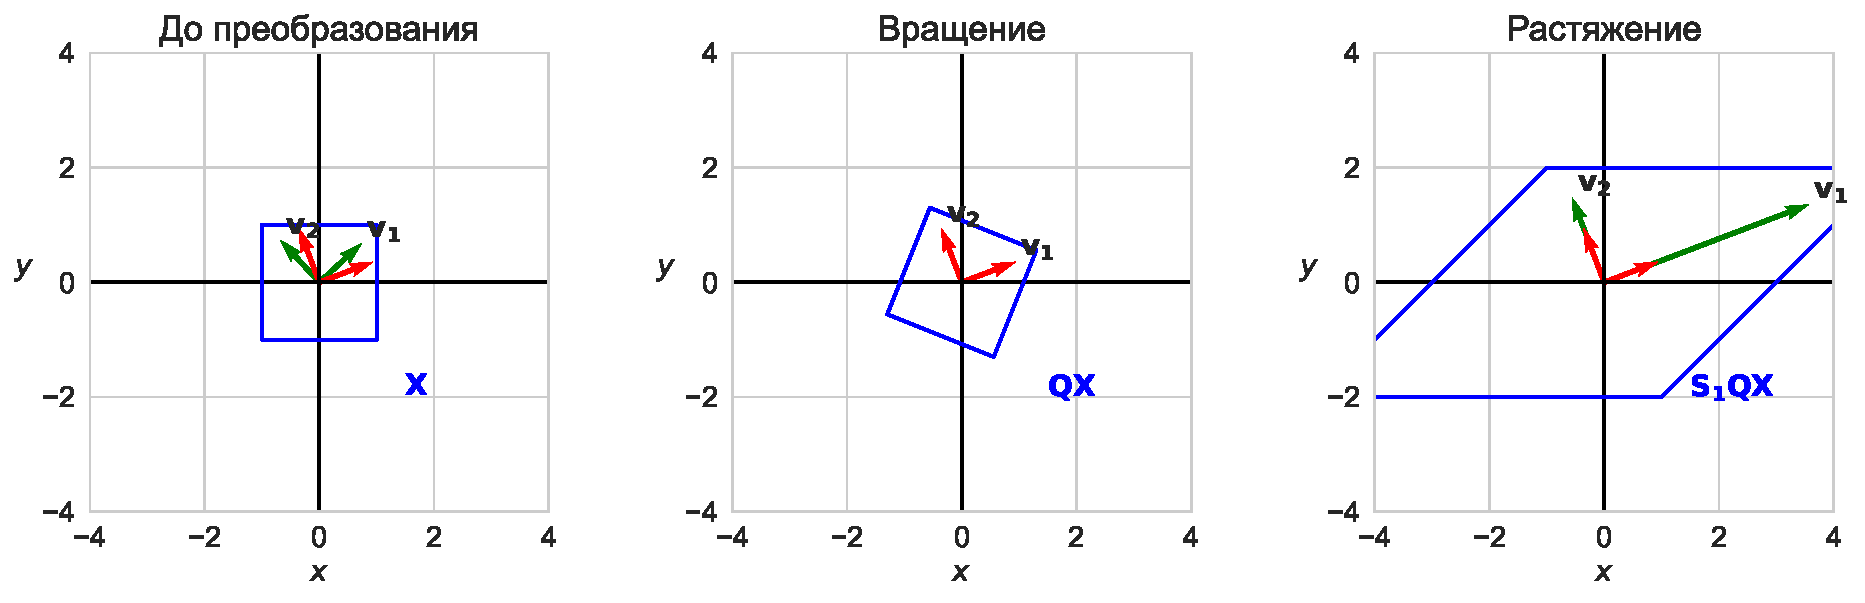
\includegraphics[width=1.0\linewidth]{Polar_1.pdf}
    \end{center}
%    { \hspace*{\fill} \\}


    \begin{tcolorbox}[breakable, size=fbox, boxrule=1pt, pad at break*=1mm,colback=cellbackground, colframe=cellborder]
\prompt{In}{incolor}{15}{\boxspacing}
\begin{Verbatim}[commandchars=\\\{\}]
\PY{n}{Q} \PY{o}{=} \PY{n}{U} \PY{o}{@} \PY{n}{Vt}
\PY{n}{S2} \PY{o}{=} \PY{n}{V} \PY{o}{@} \PY{n}{np}\PY{o}{.}\PY{n}{diag}\PY{p}{(}\PY{n}{sgm}\PY{p}{)} \PY{o}{@} \PY{n}{Vt}
\end{Verbatim}
\end{tcolorbox}

    \begin{tcolorbox}[breakable, size=fbox, boxrule=1pt, pad at break*=1mm,colback=cellbackground, colframe=cellborder]
\prompt{In}{incolor}{16}{\boxspacing}
\begin{Verbatim}[commandchars=\\\{\}]
\PY{n}{X1} \PY{o}{=} \PY{n}{S2} \PY{o}{@} \PY{n}{Sq}
\PY{n}{X2} \PY{o}{=} \PY{n}{Q} \PY{o}{@} \PY{n}{X1}
\PY{n}{Xn} \PY{o}{=} \PY{p}{[}\PY{n}{Sq}\PY{p}{,} \PY{n}{X1}\PY{p}{,} \PY{n}{X2}\PY{p}{]}
\PY{n}{Xn\PYZus{}str} \PY{o}{=} \PY{p}{[}\PY{l+s+s2}{\PYZdq{}}\PY{l+s+s2}{\PYZdl{}}\PY{l+s+s2}{\PYZbs{}}\PY{l+s+s2}{mathbf}\PY{l+s+si}{\PYZob{}X\PYZcb{}}\PY{l+s+s2}{\PYZdl{}}\PY{l+s+s2}{\PYZdq{}}\PY{p}{,} \PY{l+s+s2}{\PYZdq{}}\PY{l+s+s2}{\PYZdl{}}\PY{l+s+s2}{\PYZbs{}}\PY{l+s+s2}{mathbf}\PY{l+s+si}{\PYZob{}S\PYZus{}2X\PYZcb{}}\PY{l+s+s2}{\PYZdl{}}\PY{l+s+s2}{\PYZdq{}}\PY{p}{,} \PY{l+s+s2}{\PYZdq{}}\PY{l+s+s2}{\PYZdl{}}\PY{l+s+s2}{\PYZbs{}}\PY{l+s+s2}{mathbf}\PY{l+s+si}{\PYZob{}QS\PYZus{}2X\PYZcb{}}\PY{l+s+s2}{\PYZdl{}}\PY{l+s+s2}{\PYZdq{}}\PY{p}{]}
\PY{n}{V1} \PY{o}{=} \PY{n}{S2} \PY{o}{@} \PY{n}{V}
\PY{n}{V2} \PY{o}{=} \PY{n}{Q} \PY{o}{@} \PY{n}{V1}
\PY{n}{Vn} \PY{o}{=} \PY{p}{[}\PY{n}{V}\PY{p}{,} \PY{n}{V1}\PY{p}{,} \PY{n}{V2}\PY{p}{]}
\end{Verbatim}
\end{tcolorbox}

    \begin{tcolorbox}[breakable, size=fbox, boxrule=1pt, pad at break*=1mm,colback=cellbackground, colframe=cellborder]
\prompt{In}{incolor}{17}{\boxspacing}
\begin{Verbatim}[commandchars=\\\{\}]
\PY{n}{fig}\PY{p}{,} \PY{n}{ax} \PY{o}{=} \PY{n}{plt}\PY{o}{.}\PY{n}{subplots}\PY{p}{(}\PY{l+m+mi}{1}\PY{p}{,} \PY{l+m+mi}{3}\PY{p}{,} \PY{n}{figsize}\PY{o}{=}\PY{p}{(}\PY{l+m+mi}{15}\PY{p}{,}\PY{l+m+mi}{10}\PY{p}{)}\PY{p}{)}
\PY{n}{plt}\PY{o}{.}\PY{n}{subplots\PYZus{}adjust}\PY{p}{(}\PY{n}{wspace}\PY{o}{=}\PY{l+m+mf}{0.4}\PY{p}{)}
\PY{n}{make\PYZus{}decor}\PY{p}{(}\PY{n}{ax}\PY{p}{,} \PY{n}{xlims}\PY{p}{,} \PY{n}{ylims}\PY{p}{)}
\PY{n}{titles} \PY{o}{=} \PY{p}{[}\PY{l+s+s2}{\PYZdq{}}\PY{l+s+s2}{До преобразования}\PY{l+s+s2}{\PYZdq{}}\PY{p}{,} \PY{l+s+s2}{\PYZdq{}}\PY{l+s+s2}{Растяжение}\PY{l+s+s2}{\PYZdq{}}\PY{p}{,} \PY{l+s+s2}{\PYZdq{}}\PY{l+s+s2}{Вращение}\PY{l+s+s2}{\PYZdq{}}\PY{p}{]}

\PY{k}{for} \PY{n}{i}\PY{p}{,} \PY{n}{axi} \PY{o+ow}{in} \PY{n+nb}{enumerate}\PY{p}{(}\PY{n}{ax}\PY{o}{.}\PY{n}{flatten}\PY{p}{(}\PY{p}{)}\PY{p}{)}\PY{p}{:}
    \PY{n}{axi}\PY{o}{.}\PY{n}{plot}\PY{p}{(}\PY{n}{Xn}\PY{p}{[}\PY{n}{i}\PY{p}{]}\PY{p}{[}\PY{l+m+mi}{0}\PY{p}{,}\PY{p}{:}\PY{p}{]}\PY{p}{,} \PY{n}{Xn}\PY{p}{[}\PY{n}{i}\PY{p}{]}\PY{p}{[}\PY{l+m+mi}{1}\PY{p}{,}\PY{p}{:}\PY{p}{]}\PY{p}{,} \PY{n}{color}\PY{o}{=}\PY{l+s+s1}{\PYZsq{}}\PY{l+s+s1}{b}\PY{l+s+s1}{\PYZsq{}}\PY{p}{)}
    \PY{n}{axi}\PY{o}{.}\PY{n}{quiver}\PY{p}{(}\PY{o}{*}\PY{n}{origin}\PY{p}{,} \PY{n}{Vn}\PY{p}{[}\PY{n}{i}\PY{p}{]}\PY{p}{[}\PY{l+m+mi}{0}\PY{p}{,}\PY{p}{:}\PY{p}{]}\PY{p}{,} \PY{n}{Vn}\PY{p}{[}\PY{n}{i}\PY{p}{]}\PY{p}{[}\PY{l+m+mi}{1}\PY{p}{,}\PY{p}{:}\PY{p}{]}\PY{p}{,} \PY{n}{color}\PY{o}{=}\PY{p}{[}\PY{l+s+s1}{\PYZsq{}}\PY{l+s+s1}{g}\PY{l+s+s1}{\PYZsq{}}\PY{p}{]}\PY{p}{,}
               \PY{n}{width}\PY{o}{=}\PY{l+m+mf}{0.01}\PY{p}{,} \PY{n}{angles}\PY{o}{=}\PY{l+s+s1}{\PYZsq{}}\PY{l+s+s1}{xy}\PY{l+s+s1}{\PYZsq{}}\PY{p}{,} \PY{n}{scale\PYZus{}units}\PY{o}{=}\PY{l+s+s1}{\PYZsq{}}\PY{l+s+s1}{xy}\PY{l+s+s1}{\PYZsq{}}\PY{p}{,} \PY{n}{scale}\PY{o}{=}\PY{l+m+mi}{1}\PY{p}{)}
    \PY{n}{axi}\PY{o}{.}\PY{n}{quiver}\PY{p}{(}\PY{o}{*}\PY{n}{origin}\PY{p}{,} \PY{n}{U}\PY{p}{[}\PY{l+m+mi}{0}\PY{p}{,}\PY{p}{:}\PY{p}{]}\PY{p}{,} \PY{n}{U}\PY{p}{[}\PY{l+m+mi}{1}\PY{p}{,}\PY{p}{:}\PY{p}{]}\PY{p}{,} \PY{n}{color}\PY{o}{=}\PY{p}{[}\PY{l+s+s1}{\PYZsq{}}\PY{l+s+s1}{r}\PY{l+s+s1}{\PYZsq{}}\PY{p}{]}\PY{p}{,}
               \PY{n}{width}\PY{o}{=}\PY{l+m+mf}{0.01}\PY{p}{,} \PY{n}{angles}\PY{o}{=}\PY{l+s+s1}{\PYZsq{}}\PY{l+s+s1}{xy}\PY{l+s+s1}{\PYZsq{}}\PY{p}{,} \PY{n}{scale\PYZus{}units}\PY{o}{=}\PY{l+s+s1}{\PYZsq{}}\PY{l+s+s1}{xy}\PY{l+s+s1}{\PYZsq{}}\PY{p}{,} \PY{n}{scale}\PY{o}{=}\PY{l+m+mi}{1}\PY{p}{)}
    \PY{n}{axi}\PY{o}{.}\PY{n}{set\PYZus{}title}\PY{p}{(}\PY{n}{titles}\PY{p}{[}\PY{n}{i}\PY{p}{]}\PY{p}{)}
    \PY{n}{axi}\PY{o}{.}\PY{n}{text}\PY{p}{(}\PY{o}{*}\PY{p}{(}\PY{n}{Vn}\PY{p}{[}\PY{n}{i}\PY{p}{]}\PY{o}{.}\PY{n}{T}\PY{p}{[}\PY{l+m+mi}{0}\PY{p}{]}\PY{o}{+}\PY{p}{[}\PY{l+m+mf}{.1}\PY{p}{,}\PY{l+m+mf}{.1}\PY{p}{]}\PY{p}{)}\PY{p}{,} \PY{l+s+s2}{\PYZdq{}}\PY{l+s+s2}{\PYZdl{}}\PY{l+s+s2}{\PYZbs{}}\PY{l+s+s2}{mathbf}\PY{l+s+si}{\PYZob{}v\PYZus{}1\PYZcb{}}\PY{l+s+s2}{\PYZdl{}}\PY{l+s+s2}{\PYZdq{}}\PY{p}{,} \PY{n}{fontsize}\PY{o}{=}\PY{l+m+mi}{14}\PY{p}{)}
    \PY{n}{axi}\PY{o}{.}\PY{n}{text}\PY{p}{(}\PY{o}{*}\PY{p}{(}\PY{n}{Vn}\PY{p}{[}\PY{n}{i}\PY{p}{]}\PY{o}{.}\PY{n}{T}\PY{p}{[}\PY{l+m+mi}{1}\PY{p}{]}\PY{o}{+}\PY{p}{[}\PY{l+m+mf}{.1}\PY{p}{,}\PY{l+m+mf}{.1}\PY{p}{]}\PY{p}{)}\PY{p}{,} \PY{l+s+s2}{\PYZdq{}}\PY{l+s+s2}{\PYZdl{}}\PY{l+s+s2}{\PYZbs{}}\PY{l+s+s2}{mathbf}\PY{l+s+si}{\PYZob{}v\PYZus{}2\PYZcb{}}\PY{l+s+s2}{\PYZdl{}}\PY{l+s+s2}{\PYZdq{}}\PY{p}{,} \PY{n}{fontsize}\PY{o}{=}\PY{l+m+mi}{14}\PY{p}{)}
    \PY{n}{axi}\PY{o}{.}\PY{n}{text}\PY{p}{(}\PY{l+m+mf}{1.5}\PY{p}{,} \PY{o}{\PYZhy{}}\PY{l+m+mi}{2}\PY{p}{,} \PY{n}{Xn\PYZus{}str}\PY{p}{[}\PY{n}{i}\PY{p}{]}\PY{p}{,} \PY{n}{color}\PY{o}{=}\PY{l+s+s1}{\PYZsq{}}\PY{l+s+s1}{b}\PY{l+s+s1}{\PYZsq{}}\PY{p}{,} \PY{n}{fontsize}\PY{o}{=}\PY{l+m+mi}{14}\PY{p}{)}
\end{Verbatim}
\end{tcolorbox}

\(A = U \Sigma V^\top = \left( U V^\top \right) \left( V \Sigma V^\top \right) = QS_2\)

    \begin{center}
%      \adjustimage{max size={0.9\linewidth}{0.9\paperheight}}{Polar_2.pdf}
      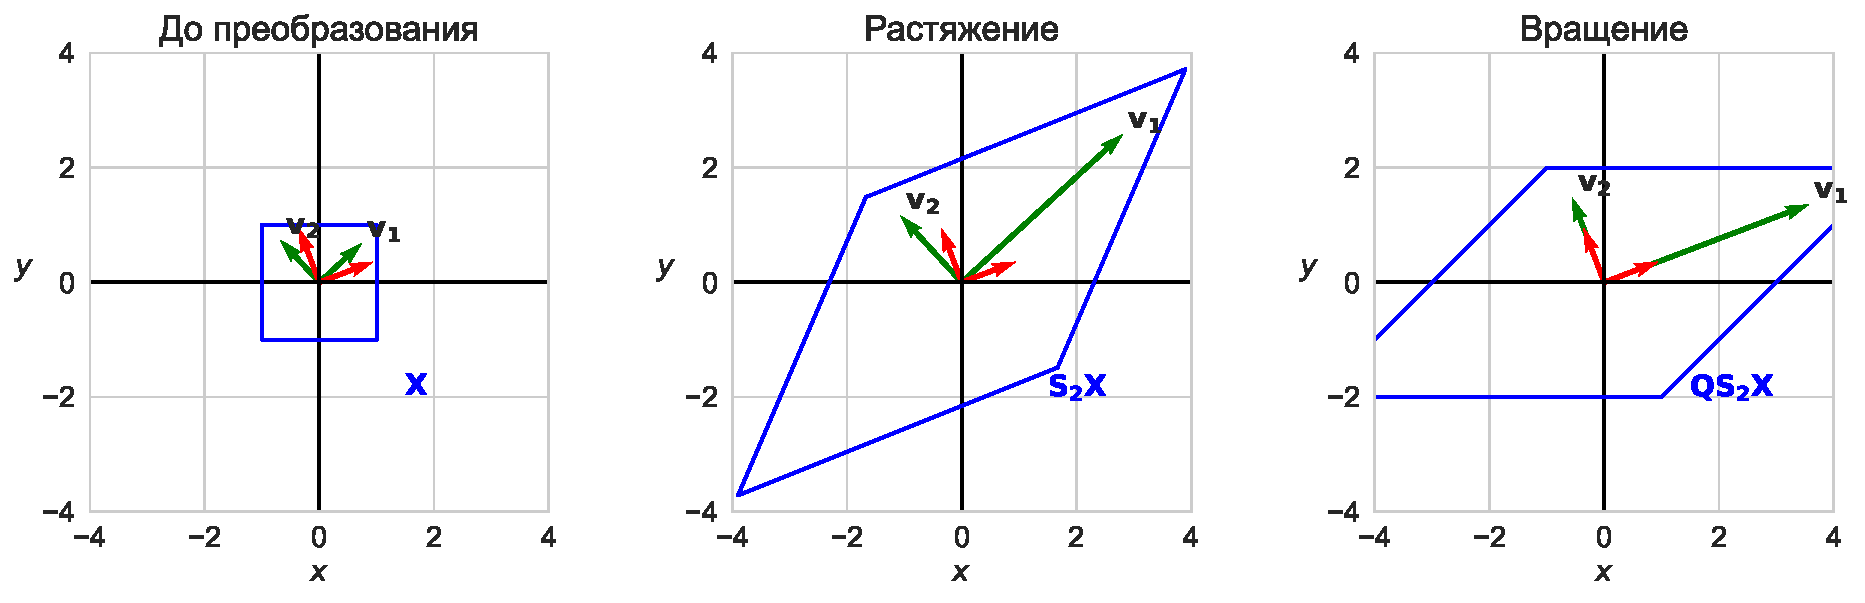
\includegraphics[width=1.0\linewidth]{Polar_2.pdf}
    \end{center}
%    { \hspace*{\fill} \\}
    
    \begin{center}\rule{0.5\linewidth}{0.5pt}\end{center}

    \hypertarget{ux438ux441ux442ux43eux447ux43dux438ux43aux438}{%
\section{Источники}\label{ux438ux441ux442ux43eux447ux43dux438ux43aux438}}

\begin{enumerate}
\def\labelenumi{\arabic{enumi}.}
\tightlist
\item
  \emph{Беклемишев Д.В.} Дополнительные главы линейной алгебры. --- М.:
  Наука, 1983. --- 336\,с.
\item
  \href{https://towardsdatascience.com/understanding-singular-value-decomposition-and-its-application-in-data-science-388a54be95d}{Материалы}
  автора \href{https://reza-bagheri79.medium.com/}{Reza Bagheri}.
\end{enumerate}

    \begin{tcolorbox}[breakable, size=fbox, boxrule=1pt, pad at break*=1mm,colback=cellbackground, colframe=cellborder]
\prompt{In}{incolor}{18}{\boxspacing}
\begin{Verbatim}[commandchars=\\\{\}]
\PY{c+c1}{\PYZsh{} Versions used}
\PY{k+kn}{import} \PY{n+nn}{sys}
\PY{n+nb}{print}\PY{p}{(}\PY{l+s+s1}{\PYZsq{}}\PY{l+s+s1}{Python: }\PY{l+s+si}{\PYZob{}\PYZcb{}}\PY{l+s+s1}{.}\PY{l+s+si}{\PYZob{}\PYZcb{}}\PY{l+s+s1}{.}\PY{l+s+si}{\PYZob{}\PYZcb{}}\PY{l+s+s1}{\PYZsq{}}\PY{o}{.}\PY{n}{format}\PY{p}{(}\PY{o}{*}\PY{n}{sys}\PY{o}{.}\PY{n}{version\PYZus{}info}\PY{p}{[}\PY{p}{:}\PY{l+m+mi}{3}\PY{p}{]}\PY{p}{)}\PY{p}{)}
\PY{n+nb}{print}\PY{p}{(}\PY{l+s+s1}{\PYZsq{}}\PY{l+s+s1}{numpy: }\PY{l+s+si}{\PYZob{}\PYZcb{}}\PY{l+s+s1}{\PYZsq{}}\PY{o}{.}\PY{n}{format}\PY{p}{(}\PY{n}{np}\PY{o}{.}\PY{n}{\PYZus{}\PYZus{}version\PYZus{}\PYZus{}}\PY{p}{)}\PY{p}{)}
\PY{n+nb}{print}\PY{p}{(}\PY{l+s+s1}{\PYZsq{}}\PY{l+s+s1}{matplotlib: }\PY{l+s+si}{\PYZob{}\PYZcb{}}\PY{l+s+s1}{\PYZsq{}}\PY{o}{.}\PY{n}{format}\PY{p}{(}\PY{n}{matplotlib}\PY{o}{.}\PY{n}{\PYZus{}\PYZus{}version\PYZus{}\PYZus{}}\PY{p}{)}\PY{p}{)}
\PY{n+nb}{print}\PY{p}{(}\PY{l+s+s1}{\PYZsq{}}\PY{l+s+s1}{seaborn: }\PY{l+s+si}{\PYZob{}\PYZcb{}}\PY{l+s+s1}{\PYZsq{}}\PY{o}{.}\PY{n}{format}\PY{p}{(}\PY{n}{seaborn}\PY{o}{.}\PY{n}{\PYZus{}\PYZus{}version\PYZus{}\PYZus{}}\PY{p}{)}\PY{p}{)}
\end{Verbatim}
\end{tcolorbox}

    \begin{Verbatim}[commandchars=\\\{\}]
Python: 3.7.11
numpy: 1.20.3
matplotlib: 3.5.1
seaborn: 0.11.2
    \end{Verbatim}



    % Add a bibliography block to the postdoc
    
    
    
\end{document}
